\documentclass[manuscript]{aomart}


\usepackage{amssymb}
\usepackage{graphicx}
\usepackage{booktabs}
\usepackage{xcolor}
\usepackage{enumitem}
\hypersetup{colorlinks=true,linkcolor=blue!50!black,citecolor=blue!50!black,urlcolor=blue!50!black,bookmarksnumbered=true,
pdftitle={Reflexive Descent to Minimal Seeds: Uniform Bounds and Free Sums},pdfauthor={Deep Bhattacharjee}}
\usepackage{tikz}
\usepackage{adjustbox}
\usepackage{placeins}
\makeatletter
\def\@aom@linecount{}
\def\@setdate{Research revision v1.3.0; \@date}
\copyrightnote{}
\makeatother
\fancyhf{}
\fancyhead[CO,CE]{\scriptsize REFLEXIVE DESCENT AND FREE SUMS}
\fancyhead[RO,LE]{\footnotesize\thepage}
\fancypagestyle{firstpage}{\fancyhf{}\renewcommand{\headrulewidth}{0pt}\cfoot{\footnotesize\thepage}}
\date{October 26, 2026}
\usepackage{microtype}

\tolerance=2000
\emergencystretch=3em
\raggedbottom

\newtheorem{theorem}{Theorem}
\newtheorem{lemma}[theorem]{Lemma}
\newtheorem{proposition}[theorem]{Proposition}
\newtheorem{corollary}[theorem]{Corollary}
\theoremstyle{definition}
\newtheorem{definition}[theorem]{Definition}
\newtheorem{conjecture}[theorem]{Conjecture}
\newtheorem{example}[theorem]{Example}
\theoremstyle{remark}
\newtheorem{remark}[theorem]{Remark}

\newcommand{\R}{\mathbb{R}}
\newcommand{\Z}{\mathbb{Z}}
\newcommand{\KS}{\mathrm{KS}}
\newcommand{\ip}[2]{\langle #1,#2\rangle}
\newcommand{\conv}{\operatorname{conv}}
\newcommand{\nvol}{\operatorname{nvol}}
\DeclareMathOperator{\Hom}{Hom}
\newcommand{\Dbig}{\Delta_{680}}
\newcommand{\UB}{348}
\newcommand{\UBplus}{349}
\newcommand{\LB}{22}
\newcommand{\DUB}{31}
\newcommand{\DepthUB}{346}



\title[Reflexive descent and free sums]{Reflexive Descent to Minimal Seeds: Uniform Bounds and Free Sums}

\author{Deep Bhattacharjee}
\address{Formerly, Electro-Gravitational Space Propulsion Laboratory (EGSPL), Bhubaneswar, Odisha 751030, India}
\address{Formerly, University of Calcutta, Senate House, 87/1 College Street, Kolkata 700073, West Bengal, India}
\email{itsdeep@live.com}
\urladdr{https://orcid.org/0000-0003-0466-750X}
\thanks{Corresponding author; second e-mail address \nolinkurl{d.bhattacharjee@erl-forschung.de}}

\thanks{The earlier joint manuscript with Ushashi Bhattacharya,
\emph{Reflexive Descent to Minimal Seeds in the Kreuzer--Skarke List},
Hexagon 2610.00456v1, supplies the preceding descent framework and
finite-dimensional certificates. Her contribution to that earlier work
is acknowledged here. This revision adds the free-sum results and
explicitly distinguishes the original results from the new checks.}

\subjclass[2020]{Primary 52B20, 14M25; Secondary 14J32, 06A07, 52-08}
\keywords{reflexive polytopes, Kreuzer--Skarke list, Calabi--Yau threefolds, lattice polytopes}

\begin{document}
\begin{abstract}
We study saturated descents through reflexive lattice subpolytopes to
r-minimal seeds. The uniform-existence conjecture has an affirmative
answer: every descent terminates, and a published volume bound gives
the classification-free estimate $D_d\le2(s_d-1)^2-2$ for $d\ge4$.
We give an exact finite construction of a descent and prove that the
reflexive-subpolytope order of a free sum in a direct-sum lattice is the
product of the factor orders. Shortest and longest descent lengths are
therefore additive. An explicit family in dimension $2r$ has shortest
length $r$ and longest length $2r$, proving that both depth and the gap
between these lengths can grow with dimension. A second base, checked
by two exact integer enumerators, gives lengths $5r$ and $6r$ and a
complete formula for the descent counts. The extremal depths are
superadditive, and $D_d/d$ has an extended limit. In dimension four the
earlier bound of $348$ for every descent remains valid; twelve interval
certificates refine the shortest-depth range to $22\le D_4\le346$
relative to the supplied Kreuzer--Skarke census. The exact value of
$D_4$ and the optimal growth rate are not determined.
\end{abstract}

\maketitle


\setcounter{tocdepth}{1}
\clearpage
\tableofcontents

\section{Introduction}\label{sec:intro}

A lattice polytope is reflexive when it contains the origin in its
interior and every facet lies on a hyperplane $\ip{x}{y}=-1$ with $y$ a
lattice vector; equivalently, its polar dual is again a lattice polytope.
Batyrev showed that a reflexive polytope $\Delta$ of dimension four gives a
family of Calabi--Yau threefolds, the anticanonical hypersurfaces in the
toric variety of the fan over the faces of $\Delta^*$, and that the
exchange of $\Delta$ and $\Delta^*$ is mirror symmetry~\cite{Bat94}.
Kreuzer and Skarke classified these polytopes: there are $16$ in dimension
two, $4{,}319$ in dimension three~\cite{KS98} and $473{,}800{,}776$ in
dimension four~\cite{KS00}, up to unimodular equivalence. We write $\KS_d$
for the list in dimension $d$.

The classification rests on a finiteness principle. A lattice polytope with
the origin in its interior is called \emph{minimal} when removing any one
of its vertices and taking the convex hull of the others loses that
property, and every reflexive polytope contains a minimal one spanned by
some of its vertices~\cite{KS97,KS00}. In dimension four Kreuzer and
Skarke worked with a sharper notion: a reflexive polytope is
\emph{r-minimal} when it contains no reflexive polytope other than itself,
and every reflexive polytope contains an r-minimal one. Both notions
describe the seeds from which the whole list is grown, and the question
studied here is how far a polytope is from its seeds.

The seed universality preprint~\cite{Bha26a} proposed that the list is
generated from at most $64$ seed orbits with Hodge numbers constant on each
orbit. A later note~\cite{Bha26b} refuted that proposal, kept what is true
near it, and isolated the following statement as the part that remained
open.

\begin{conjecture}[Uniform transition depth~\cite{Bha26b}]\label{conj:depth}
There is an absolute constant $D$ such that every $\Delta\in\KS_4$ is
connected to some minimal seed by a chain of at most $D$ subpolytope steps
$\Delta_i\supset\Delta_{i+1}$ in which every intermediate hull is
reflexive after unimodular equivalence. The stratification data suggest a
value of $D$ of order a few tens.
\end{conjecture}

The assertion of a uniform constant is already settled by the finite-order
argument below; it is distinct from determining the sharp constant or
justifying the heuristic of a few tens. This revision gives a further,
classification-free construction for varying dimensions.

The note also asserted that descent through reflexive polytopes alone is
not always possible, and offered a vertex-deletion chain with
non-reflexive intermediate hulls as the substitute. We show that the
assertion is false, prove the conjecture with an explicit constant, and
determine the constant exactly in dimensions two and three.

To make the statement precise we use the order of the reflexive polytopes
by inclusion. A reflexive polytope $\Gamma\subsetneq\Delta$ is a
\emph{cover} of $\Delta$ when no reflexive polytope lies strictly between
them.\footnote{Here and below all polytopes live in the same lattice $M$
and have the origin as their only interior lattice point; a subpolytope of
$\Delta$ is a lattice polytope contained in $\Delta$. Reflexivity of a
subpolytope is always meant with respect to $M$ and the origin, which is
the reading of ``after unimodular equivalence'' in
Conjecture~\ref{conj:depth}: a unimodular map that carries $\Gamma$ into
$\Delta$ fixes the origin and the lattice.} A \emph{reflexive descent} of
$\Delta$ is a chain
\[
\Delta=\Delta_0\supsetneq\Delta_1\supsetneq\cdots\supsetneq\Delta_k
\]
in which each $\Delta_{i+1}$ is a cover of $\Delta_i$ and $\Delta_k$ is
r-minimal. Its length is $k$, and the \emph{transition depth}
$\delta(\Delta)$ is the least length of a reflexive descent of $\Delta$.
A descent never skips a reflexive polytope, so it is the strictest form of
the chains in Conjecture~\ref{conj:depth}; without the cover condition
every polytope reaches a seed in one step, as we explain in
Section~\ref{sec:literal}. We write $D_d$ for the largest transition depth
in $\KS_d$, and $|P|$ for the number of lattice points of a polytope $P$.
For arbitrary dimension, $D_d$ denotes the maximum over all reflexive
$d$-polytopes; no classified list in dimension greater than four is
assumed. Its finiteness also follows from Proposition~\ref{prop:everydim}.

\begin{theorem}\label{thm:A}
Every reflexive polytope has a reflexive descent, every reflexive descent
ends at an r-minimal polytope, and every r-minimal polytope contains a
minimal polytope. Hence every $\Delta\in\KS_4$ is joined to a minimal seed
by a chain in which every intermediate hull is reflexive and no reflexive
polytope fits between two consecutive members.
\end{theorem}

\begin{theorem}\label{thm:B}
No reflexive descent in dimension four has more than $\UB$ steps. More
precisely, every reflexive descent of $\Delta\in\KS_4$ has length at most
$\min(|\Delta|-6,\,680-|\Delta^*|)$ and at most the pair bound
$L(|\Delta|,|\Delta^*|)$ of Section~\ref{sec:counting}. The first number
never exceeds $654$ and the second never exceeds $\UB$, and each maximum
is attained by a single polytope. Hence $D_4\le\UB$, and
Conjecture~\ref{conj:depth} holds with $D=\UBplus$.
\end{theorem}

\begin{theorem}\label{thm:C}
$D_2=5$ and $D_3=11$. In dimension two the maximum is attained only by the
triangle with ten lattice points; in dimension three it is attained by
exactly two polytopes, with $35$ and $31$ lattice points, both of which are
contained in no larger reflexive polytope.
\end{theorem}

\begin{theorem}\label{thm:D}
The polytopes $P_1$ and $P_2$ of Section~\ref{ssec:depth22}, with $37$
lattice points each, have transition depth exactly $\LB$, and $P_1$ is
unimodularly equivalent to the polytope reached after ten steps of a
reflexive descent of the simplex $\Dbig$ with $680$ lattice points, the
largest reflexive polytope in dimension four. The transition depth of
$\Dbig$ is at most $\DUB$. Hence $\LB\le D_4\le\UB$.
\end{theorem}

Theorem~\ref{thm:B} bounds every descent, not only the shortest one, so it
also bounds the longest chain of covers below any polytope. The existence
of some constant $D$ is the easy part of the conjecture: the list is finite
and Theorem~\ref{thm:A} gives each polytope a descent. The content of
Theorem~\ref{thm:B} is that the constant can be read off from two numbers
attached to each polytope, its lattice points and the lattice points of
its dual, without examining any polytope. The same count, with
Blichfeldt's bound on lattice points and the volume theorem of Balletti,
Kasprzyk and Nill in place of the list, bounds the depth in every
dimension: $D_d\le2(s_d-1)^2-2$ for $d\ge4$, where $s_d$ is Sylvester's
sequence (Proposition~\ref{prop:everydim}). The guess of ``a few tens'' in
the conjecture is neither confirmed nor refuted. The exact values $5$ and
$11$ in lower dimension, the depth $\LB$ of two polytopes with thirty-seven
points and the descent of length $\DUB$ from the largest polytope are
consistent with it. The interval refinement in Corollary~\ref{cor:seed346}
gives $\LB\le D_4\le\DepthUB$ relative to the supplied census;
the exact value remains open.

Theorem~\ref{thm:A} is a short argument in the inclusion order
(Section~\ref{sec:literal}). Theorem~\ref{thm:B} counts lattice points on
both sides of the duality: along a descent the polytope loses points and
its dual gains them, and both counts must stay among the pairs that occur
in the list (Section~\ref{sec:counting}). For the lower bounds we need all
covers of a given polytope. Section~\ref{sec:cuts} describes them as cuts
along dual lattice points; the volume bound of Balletti, Kasprzyk and
Nill~\cite{BKN22} leaves finitely many cuts to try, and a climbing lemma
certifies one cover without listing the others. In dimension two these
tools give $D_2=5$ by hand, and in dimensions three and four they give the
exact values and constructions of Sections~\ref{sec:low}
and~\ref{sec:four}. A lower bound for a depth is a statement about every
descent, and in dimension four we prove it with a certificate: a finite set
of polytopes with their complete lists of covers and a bound attached to
each, subject to a condition that can be checked one polytope at a time
(Lemma~\ref{lem:certificate}). The polytopes $P_1$ and $P_2$ are skew
bipyramids over a three-dimensional reflexive tetrahedron, and their
certificate contains $5{,}592$ polytopes. Section~\ref{sec:open} lists what
remains open.

\begin{theorem}[Free-sum construction]\label{thm:intro-free}
For reflexive polytopes $P,Q$ in direct-sum lattices,
\[
 R(P\oplus Q)\cong R(P)\times R(Q),\qquad
 \delta(P\oplus Q)=\delta(P)+\delta(Q).
\]
The analogous equality holds for longest descent lengths. In particular,
explicit polytopes of dimension $2r$ have shortest and longest lengths
$r$ and $2r$; a second independently checked base gives $5r$ and $6r$.
The maxima satisfy $D_{m+n}\ge D_m+D_n$.
\end{theorem}

These statements are proved in Section~\ref{sec:freesums}. The first
family has a five-element planar subpolytope order, verified directly
by primitive facet inequalities, so it needs neither a census nor a
computational certificate. It answers the question about the existence
of a growing lower bound from the earlier manuscript~\cite{Joint26}.
The second family's base profile is exhaustively checked over $512$
subsets by two integer implementations. These are polytope descent
results; they do not construct a string vacuum or settle GSC.

\subsection*{History}

Reflexive polytopes entered algebraic geometry through Batyrev's
construction of mirror pairs of Calabi--Yau hypersurfaces~\cite{Bat94};
the lattice-point formulas for $h^{1,1}$ and $h^{2,1}$ in that paper made
the polytopes themselves the objects of study. Kreuzer and Skarke set out
to list them. Their first paper~\cite{KS97} introduced the minimal
polytopes, showed that a minimal polytope is either a simplex or a union of
lower-dimensional simplices sharing the origin as an interior point, and
attached a weight system to each simplex, so that the minimal polytopes in
a given dimension come from finitely many combined weight systems. The
three-dimensional list of $4{,}319$ polytopes followed in
1998~\cite{KS98}. In dimension four the combined weight systems number
$201{,}346$, too many to use directly, and Kreuzer and Skarke replaced
minimality by r-minimality: only $308$ combined weight systems give
r-maximal polytopes, that is, duals of r-minimal ones, and together with
$25$ sublattice versions and $7$ exceptional polytopes they give the $340$
r-maximal reflexive polytopes of dimension four~\cite{KS00}. Every
reflexive four-polytope is a subpolytope of one of these, and the complete
list of $473{,}800{,}776$ was obtained by enumerating subpolytopes with the
program PALP~\cite{KS04}. The lattice-point counts range from $6$ to
$680$~\cite{KS00}.

The inclusion order was used from the start to argue that the Calabi--Yau
hypersurfaces form a connected web. Candelas, Green and H\"ubsch had shown
that the complete intersections in products of projective spaces are
connected by conifold transitions~\cite{CGH90}; Avram, Kreuzer, Mandelberg
and Skarke showed that the toric hypersurfaces from weighted projective
spaces form a web connected by inclusions of polytopes~\cite{AKMS97}; and
Kreuzer and Skarke observed that connectedness of all reflexive
four-polytopes reduces to connectedness of the $340$ r-maximal ones, which
they checked during the classification~\cite{KS00}. Reid's question whether
all Calabi--Yau threefolds lie in one family connected by such
transitions~\cite{Rei87} remains open in general. Databases built on the
list~\cite{AGHJN15} made the joint statistics of polytopes and Hodge
numbers easy to read, and the list is now distributed in a form that can be
streamed in a few minutes~\cite{HF4D}.

The extremes of the list have a separate history. Lagarias and Ziegler
bounded the volume of lattice polytopes with a fixed number of interior
points~\cite{LZ91}; for reflexive polytopes the sharp bound was proved by
Balletti, Kasprzyk and Nill~\cite{BKN22}, who showed that in every
dimension $d\ge4$ the largest reflexive polytope is a simplex built from
Sylvester's sequence. In dimension four it is the simplex $\Dbig$ with
$680$ lattice points, the Newton polytope of the hypersurface of degree
$84$ in the weighted projective space $\mathbb{P}(1,1,12,28,42)$, whose
mirror is the Calabi--Yau threefold with the largest value of $h^{1,1}$ in
the list.

The question of distance to the seeds came from the seed universality
preprint~\cite{Bha26a}. Its orbit picture combined polar duality, stellar
subdivision and flips, and claimed constant Hodge numbers on at most $64$
orbits; the correcting note~\cite{Bha26b} disposed of that claim with two
observations (duality exchanges the Hodge pairs $(1,101)$ and $(101,1)$ of
the quintic and its mirror, and the list realises $30{,}108$ Hodge pairs),
proved the statements that survive at a fixed polytope, and stated
Conjecture~\ref{conj:depth}. The present paper answers it. Related work of
the first author on Calabi--Yau geometry and the landscape
includes~\cite{Bha26c}.

\section{Reflexive polytopes and their order}\label{sec:prelim}

Let $M\cong\Z^d$ be a lattice, $N=\Hom(M,\Z)$ its dual and
$\ip{\cdot}{\cdot}$ the pairing. For a polytope $P\subset M_\R$ with the
origin in its interior the polar dual is
$P^*=\{y\in N_\R:\ip{x}{y}\ge-1\text{ for all }x\in P\}$. A lattice polytope
$\Delta$ is reflexive when $\Delta^*$ is a lattice polytope; then
$\Delta^{**}=\Delta$, the facets of $\Delta$ are the sets
$\{\ip{x}{v}=-1\}\cap\Delta$ for the vertices $v$ of $\Delta^*$, and the
origin is the only interior lattice point. For a reflexive $\Delta$ let
$R(\Delta)$ be the set of reflexive subpolytopes of $\Delta$.

\begin{lemma}\label{lem:basic}
Let $\Gamma\subsetneq\Delta$ be lattice polytopes with the origin in their
interiors. Then
\begin{enumerate}[label=\textup{(\roman*)},leftmargin=*]
\item $|\Gamma|<|\Delta|$;
\item $\Delta^*\subsetneq\Gamma^*$, and if both are reflexive then
$|\Delta^*|<|\Gamma^*|$;
\item $R(\Delta)$ is finite, and every element of $R(\Delta)$ other than
$\Delta$ lies in a cover of $\Delta$.
\end{enumerate}
\end{lemma}

\begin{proof}
(i) If every vertex of $\Delta$ lay in $\Gamma$, the convex hull $\Delta$
would lie in $\Gamma$; so some vertex of $\Delta$, a lattice point, is
missing from $\Gamma$. (ii) Polarity reverses inclusion and is injective
on polytopes with the origin inside, and (i) applies to the lattice
polytopes $\Delta^*\subsetneq\Gamma^*$. (iii) A reflexive subpolytope is
the convex hull of a set of lattice points of $\Delta$, so there are at
most $2^{|\Delta|}$ of them. Given $\Gamma\in R(\Delta)$ with
$\Gamma\ne\Delta$, a maximal element of
$\{\Gamma'\in R(\Delta):\Gamma\subseteq\Gamma'\ne\Delta\}$ exists by
finiteness and is a cover of $\Delta$.
\end{proof}

A polytope is r-minimal exactly when it has no cover. By
Lemma~\ref{lem:basic}(iii) a reflexive polytope that is not r-minimal has
at least one cover, and we will need all of them.

\section{The literal conjecture and reflexive descent}\label{sec:literal}
\enlargethispage{4pt}

\begin{proof}[Proof of Theorem~\ref{thm:A}]
Let $\Delta$ be reflexive. If $\Delta$ is r-minimal the descent of length
zero will do. Otherwise Lemma~\ref{lem:basic}(iii) gives a cover
$\Delta_1$, and we repeat with $\Delta_1$. By Lemma~\ref{lem:basic}(i) the
number of lattice points drops at each step, so the process stops, and it
stops exactly at an r-minimal polytope. Any reflexive descent ends at an
r-minimal polytope by definition.

Let $\Delta_k$ be r-minimal and let $V$ be its vertex set. Remove vertices
from $V$ one at a time, keeping the origin in the interior of the convex
hull of what is left, until no vertex can be removed. The hull $S$ of the
remaining set is a minimal polytope, its vertices are vertices of
$\Delta_k$, and $S\subseteq\Delta_k$. If $S\ne\Delta_k$ the step
$\Delta_k\supsetneq S$ leaves no room for a reflexive polytope between the
two, because $\Delta_k$ has no reflexive subpolytope other than itself.
Appending this step to a reflexive descent gives the chain of the
theorem.
\end{proof}

Three readings of Conjecture~\ref{conj:depth} are now settled at once. If
a ``subpolytope step'' may be any inclusion, the chain
$\Delta\supsetneq S$ of the second paragraph applied to $\Delta$ itself
has no intermediate hull at all, and $D=1$; this is the minimal-polytope
theorem of Kreuzer and Skarke~\cite{KS97} restated. If the seeds are the
r-minimal polytopes, which are the seeds of the four-dimensional
classification~\cite{KS00}, a reflexive descent ends at a seed. If the
seeds are minimal polytopes, at most one further step is needed. In every
reading the chain length is controlled by the transition depth, which is
the quantity bounded in Theorem~\ref{thm:B}.\footnote{In dimensions two and
three we checked which r-minimal polytopes are themselves minimal. The
three r-minimal polygons are minimal; in dimension three, twelve of the
sixteen r-minimal polytopes are minimal and four contain a smaller
minimal polytope that is not reflexive. In dimension four Kreuzer and
Skarke found seven r-minimal polytopes that do not come from weight
systems, and each of them contains a single minimal subpolytope, a simplex
that is not reflexive~\cite{KS00}.}

The correcting note~\cite{Bha26b} stated that descent through reflexive
polytopes only is not always possible. Theorem~\ref{thm:A} shows that it
always is. What fails is descent by deleting vertices, which is the
operation the note had in mind, and it fails in two ways.

\begin{proposition}\label{prop:vertexdeletion}
\begin{enumerate}[label=\textup{(\roman*)},leftmargin=*]
\item If $\Delta$ is a reflexive simplex, the convex hull of any proper
subset of its vertices is a face of $\Delta$ and contains no interior
point; so a reflexive simplex that is not r-minimal admits no descent by
convex hulls of vertex subsets, although it has a reflexive descent.
\item Among the $4{,}303$ reflexive three-polytopes that are not
r-minimal, exactly $74$ have no reflexive subpolytope of the form
$\conv\bigl((\Delta\cap M)\setminus\{v\}\bigr)$ with $v$ a vertex, and
exactly $354$ have none of the form $\conv(V\setminus\{v\})$ with $V$ the
vertex set.
\end{enumerate}
\end{proposition}

\begin{proof}
Part (i) is immediate: a proper subset of the vertices of a simplex spans
a face of positive codimension. Part (ii) is a finite check on the list of
Kreuzer and Skarke, recorded in the code archive~\cite{Repo}.
\end{proof}

\begin{example}\label{ex:vertexdeletion}
The smallest polytope in part (ii) has $15$ lattice points and vertices
$(1,0,0)$, $(0,1,0)$, $(-1,-1,0)$, $(0,0,1)$, $(-3,2,-2)$, $(-2,3,-2)$,
$(-4,4,-3)$. Removing any one vertex and taking the hull of the remaining
fourteen lattice points gives a polytope that is not reflexive, yet the
polytope has a reflexive descent of length $5$. In dimension four the
largest polytope $\Dbig$ is a simplex, so by part (i) it cannot be reduced
by vertex deletion at all, while Theorem~\ref{thm:D} gives it a descent of
length $\DUB$.
\end{example}

The vertex-deletion chain of the note does reach a minimal polytope, and
its length is less than the number of vertices~\cite{Bha26b}; in dimension
four the vertex counts range from $5$ to $33$~\cite{KS00}, so such chains
have at most $28$ steps. Its intermediate hulls are not reflexive in
general, which is why the conjecture was stated with reflexive
intermediates.

\section{Counting lattice points}\label{sec:counting}
\enlargethispage{4pt}

The lattice points of a polytope and of its dual move in opposite
directions along a descent, and in dimension four both counts are known for
every polytope of the list. This is enough to bound the length of every
descent. We write $\mathcal{P}_4\subset\Z^2$ for the set of pairs
$(|\Delta|,|\Delta^*|)$ with $\Delta\in\KS_4$; both numbers are invariant
under unimodular maps, and $\mathcal{P}_4$ is symmetric under
$(p,q)\mapsto(q,p)$ because the list is closed under duality.

\begin{definition}\label{def:pairbound}
For $(p,q)\in\mathcal{P}_4$ let $L(p,q)$ be the largest $k$ for which
there are pairs $(p_0,q_0),\dots,(p_k,q_k)$ in $\mathcal{P}_4$ with
$(p_0,q_0)=(p,q)$, $p_0>p_1>\cdots>p_k$ and $q_0<q_1<\cdots<q_k$. We call
$L(p,q)$ the \emph{pair bound} and write $L(\Delta)=L(|\Delta|,|\Delta^*|)$.
\end{definition}

The pair bound satisfies $L(p,q)=1+\max L(p',q')$ over the pairs with
$p'<p$ and $q'>q$, and $L(p,q)=0$ when there is no such pair. Evaluating
this recursion in increasing order of $p$ computes $L$ on all of
$\mathcal{P}_4$ at once.

\begin{lemma}\label{lem:counting}
Let $\Delta_0\supsetneq\Delta_1\supsetneq\cdots\supsetneq\Delta_k$ be
reflexive polytopes of dimension four, not necessarily a descent. Then
\[
k\;\le\;L(\Delta_0)\;\le\;\min\bigl(|\Delta_0|-6,\;680-|\Delta_0^*|\bigr).
\]
\end{lemma}

\begin{proof}
By Lemma~\ref{lem:basic} the counts $|\Delta_i|$ strictly decrease and the
counts $|\Delta_i^*|$ strictly increase. Each $\Delta_i$ is unimodularly
equivalent to a member of $\KS_4$, so each pair
$(|\Delta_i|,|\Delta_i^*|)$ lies in $\mathcal{P}_4$, and the pairs form a
chain as in Definition~\ref{def:pairbound}. Hence $k\le L(\Delta_0)$. In
any such chain of pairs the first coordinates are distinct integers between
$p_k$ and $p_0$ and the second are distinct integers between $q_0$ and
$q_k$. Every reflexive polytope of dimension four has at least six lattice
points and at most $680$~\cite{KS00}, which gives the second
inequality.\footnote{The lower bound six is elementary: a full-dimensional
lattice polytope in dimension four with an interior point has at least five
vertices, and the origin is a further lattice point. The upper bound $680$
is attained only by the simplex $\Dbig$ of Section~\ref{sec:four}, as the
list shows; Balletti, Kasprzyk and Nill proved that this simplex also has
the largest volume among reflexive four-polytopes~\cite{BKN22}.}
\end{proof}

The set $\mathcal{P}_4$ was computed by reading the two point counts of
all $473{,}800{,}776$ polytopes of the list~\cite{HF4D}. It has $71{,}870$
elements, its extreme values $6$ and $680$ agree with those recorded by
Kreuzer and Skarke~\cite{KS00}, and the counts add up to the size of the
list. Table~\ref{tab:counting} and Fig.~\ref{fig:pairs} summarise both
bounds over the list.

\begin{table}[t]
\caption{Number of polytopes in $\KS_4$ whose bound on the length of a
reflexive descent exceeds a given value, for the simple bound
$\min(|\Delta|-6,680-|\Delta^*|)$ and for the pair bound $L(\Delta)$. The
note below the table gives the largest value of each bound and the point pair where it
is attained.}\label{tab:counting}
\centering
\begin{adjustbox}{max width=\linewidth}\begin{tabular}{lrr}
\toprule
bound exceeds & $\min(|\Delta|-6,680-|\Delta^*|)$ & $L(\Delta)$\\
\midrule
$100$ & $7{,}159{,}636$ & $6{,}838{,}181$\\
$150$ & $893{,}324$ & $825{,}559$\\
$200$ & $136{,}519$ & $117{,}767$\\
$250$ & $30{,}306$ & $23{,}814$\\
$300$ & $7{,}755$ & $3{,}556$\\
$320$ & $4{,}763$ & $1{,}028$\\
$340$ & $2{,}705$ & $106$\\
$348$ & $2{,}197$ & $0$\\
$500$ & $39$ & $0$\\
$654$ & $0$ & $0$\\
\bottomrule
\end{tabular}\end{adjustbox}
\par\smallskip
\parbox{0.9\textwidth}{\small\raggedright simple bound $654$ at $(680,26)$, the simplex $\Dbig$; pair bound $348$ at $(521,22)$, a single polytope with seven vertices.}
\end{table}

\begin{figure}[t]
\centering
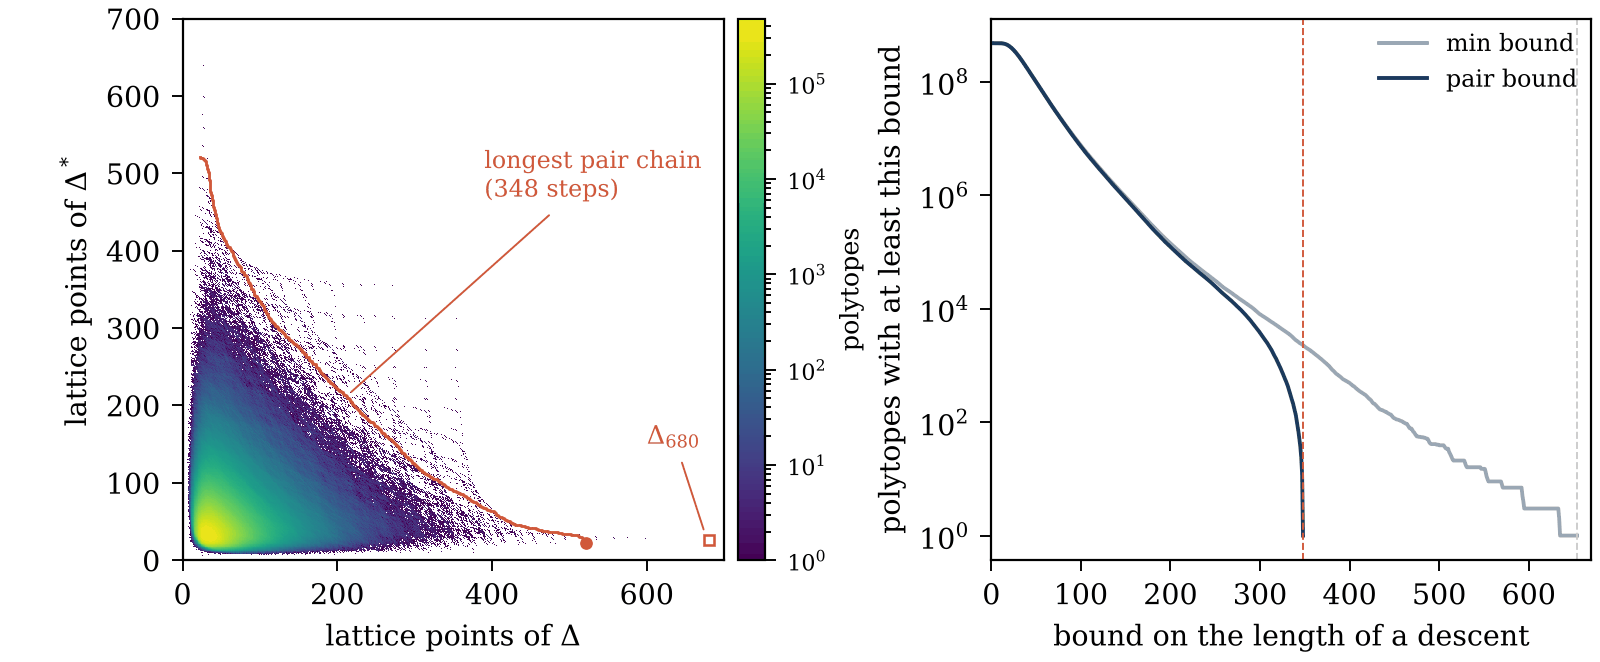
\includegraphics[width=\textwidth]{figures/fig_pairs.png}
\caption{Left: the number of reflexive four-polytopes with a given number
of lattice points (horizontal) and dual lattice points (vertical), on a
logarithmic colour scale. A reflexive descent moves left and up through
occupied cells. The red staircase is a longest chain of occupied cells,
with $348$ steps from $(521,22)$ to its mirror image $(22,521)$; the dot
marks its start and the square marks the simplex $\Dbig$ at $(680,26)$.
Right: for each value $X$, the number of polytopes whose bound on the
length of a descent is at least $X$, for the simple bound and the pair
bound.}\label{fig:pairs}
\end{figure}

\begin{proof}[Proof of Theorem~\ref{thm:B}]
Lemma~\ref{lem:counting} applies to every reflexive descent. Over
$\mathcal{P}_4$ the largest value of $\min(p-6,680-q)$ is $654$, attained
only at $(680,26)$, and this pair belongs to one polytope, the simplex
$\Dbig$; the next values are $634$ at $(640,26)$ and $633$ at $(639,27)$.
The largest value of $L$ is $348$, attained only at $(521,22)$, again by a
single polytope, with vertices
\begin{multline*}
(1,0,0,0),\ (0,1,0,0),\ (0,0,1,0),\ (1,1,1,2),\\
(-3,-3,1,-2),\ (-45,-38,-6,-30),\ (15,22,-6,30)
\end{multline*}
and Hodge numbers $(h^{1,1},h^{2,1})=(10,376)$ for the hypersurface of
which it is the Newton polytope. So every reflexive descent in dimension
four has at most $\UB$ steps, $D_4\le\UB$, and with one more step to a
minimal polytope (Theorem~\ref{thm:A}) Conjecture~\ref{conj:depth} holds
with $D=\UBplus$.
\end{proof}

The pair bound of $\Dbig$ is $347$. A longest chain of pairs from
$(521,22)$ runs close to the upper edge of the occupied region and ends at
the mirror pair $(22,521)$ (Fig.~\ref{fig:pairs}). The chain is a property
of the point counts only; nothing in the argument says that a descent
follows it, and the descents we can compute are much shorter. For the
polytope at $(521,22)$, two covers found by the method of the next section
lead to a polytope with $257$ lattice points and $24$ dual points, whose
pair bound is $247$, so that polytope has a descent of length at most
$249$.

\begin{corollary}\label{cor:347}
The maximum shortest reflexive-descent depth satisfies $22\le D_4\le347$.
\end{corollary}
\begin{proof}
The unique polytope whose pair bound is $348$ has a chain of two covers
with point-count pairs $(521,22)$, $(516,23)$, $(257,24)$. The final pair
has bound $247$, so this polytope has shortest depth at most $2+247=249$.
Every other polytope has pair bound at most $347$. The lower bound $22$
is unchanged. The certificate and an integer-arithmetic verifier are
\texttt{code/data/top347\_certificate.json} and
\texttt{code/checks/check\_top347.py}. This sharpens the bound for shortest
descents; the bound $348$ for arbitrary descents is unchanged.
\end{proof}


\subsection{Twelve interval certificates for shorter descents}\label{ssec:seedinterval}
\begin{lemma}\label{lem:seedinterval}
For reflexive polytopes $Q\subsetneq P$ in a fixed lattice,
\[
 \delta(P)\le \min\{|P|-|Q|,\ |Q^*|-|P^*|\}+\delta(Q).
\]
In dimension four the last term can be replaced by the pair bound
$L(|Q|,|Q^*|)$. The inclusion $Q\subsetneq P$ need not be a cover.
\end{lemma}
\begin{proof}
Choose a maximal chain in the finite interval $[Q,P]$ of reflexive
subpolytopes. Any reflexive polytope strictly between consecutive
members would also belong to that interval, so each step is a cover
in the whole reflexive inclusion order. At each step at least one
primal point is lost and at least one dual point is gained, by
Lemma~\ref{lem:basic}. The chain length is bounded by both differences.
Concatenate it with a shortest descent of $Q$. The pair-bound version
uses Lemma~\ref{lem:counting} for the final descent.
\end{proof}

\begin{corollary}[Finite-census refinement]\label{cor:seed346}
Relative to the supplied Kreuzer--Skarke point-pair census and the
published classification, the maximum shortest depth satisfies
$22\le D_4\le346$. The arbitrary-descent bound remains $348$.
\end{corollary}
\begin{proof}
Compute $L(p,q)=\max(\{0\}\cup\{1+L(p',q'):p'<p,\ q'>q\})$
over the occupied pairs, batching updates with equal $p$.
Exactly twelve census entries have $L>346$. The following strict
reflexive intervals cover these entries; $c$ is the minimum of the
two point-count differences in Lemma~\ref{lem:seedinterval}.
\begin{center}\small
\begin{adjustbox}{max width=\linewidth}\begin{tabular}{rrrrr}\toprule
$(|P|,|P^*|)$ & $(|Q|,|Q^*|)$ & $c$ & $L(Q)$ & $c+L(Q)$\\\midrule
$(445,17)$ & $(112,22)$ & 5 & 105 & 110\\
$(680,26)$ & $(422,27)$ & 1 & 339 & 340\\
$(640,26)$ & $(400,27)$ & 1 & 338 & 339\\
$(600,26)$ & $(378,27)$ & 1 & 326 & 327\\
$(560,26)$ & $(356,27)$ & 1 & 325 & 326\\
$(576,26)$ & $(360,27)$ & 1 & 326 & 327\\
$(520,26)$ & $(334,27)$ & 1 & 315 & 316\\
$(520,26)$ & $(325,27)$ & 1 & 308 & 309\\
$(516,23)$ & $(181,25)$ & 2 & 173 & 175\\
$(521,22)$ & $(181,25)$ & 3 & 173 & 176\\
$(536,26)$ & $(338,27)$ & 1 & 316 & 317\\
$(482,22)$ & $(168,25)$ & 3 & 161 & 164\\
\bottomrule\end{tabular}\end{adjustbox}
\end{center}
The stored vertices and integral cut vectors specify each interval.
The exact checker reconstructs every facet and every lattice point of
$P,Q,P^*,Q^*$, verifies reflexivity and strict containment, and checks
that the cut yields exactly the child's point set. It verifies the
exceptional multiset against the census. The two representatives at
$(520,26)$ have different multisets of absolute four-by-four vertex
determinants, proving that they are not unimodularly equivalent; the
other ten representatives have distinct point pairs. Thus the twelve
representatives exhaust the exceptional classes under the supplied
census counts. All displayed bounds are below $346$; every remaining
pair has $L\le346$. The earlier depth-$22$ certificate supplies the
lower bound.
\end{proof}
The certificate records the histogram digest, vertices, primal points,
cut vectors and coordinate-source digests. The verifier uses integer
arithmetic and does not assert that these cuts are covers. Its output
was rechecked for this revision. It uses the supplied histogram; it
does not rederive the classification or rescan all $473{,}800{,}776$
coordinate records. This distinction is separate from the completely
analytic uniform bound and free-sum construction.

In other dimensions the joint distribution of point counts is not known,
but the extremes are, and they already bound the depth. Let
$s_1=2$ and $s_{k+1}=s_k^2-s_k+1$ be Sylvester's sequence, so that
$s_2,s_3,s_4,s_5=3,7,43,1807$.

\begin{proposition}\label{prop:everydim}
Let $V_d$ be the largest normalised volume of a reflexive polytope of
dimension $d$. Every chain
$\Delta_0\supsetneq\Delta_1\supsetneq\cdots\supsetneq\Delta_k$ of
reflexive polytopes of dimension $d$ has
\[
k\;\le\;V_d-2 .
\]
In particular $D_d\le V_d-2$ for every $d\ge2$, and
$D_d\le2(s_d-1)^2-2$ for every $d\ge4$.
\end{proposition}

\begin{proof}
We include the lattice-point argument rather than leaving Blichfeldt's
inequality~\cite{Bli14} as an additional input. Triangulate a
full-dimensional lattice polytope $P$ with every point of $P\cap M$ as
a vertex. Such a triangulation is obtained by an initial triangulation
and successive stellar insertions of the remaining finite set of points.
Let $t$ be its number of full-dimensional simplices. Their facet-adjacency
graph is connected: a generic path in the interior between two simplex
interiors crosses only their facets. Order the simplices by traversing
a spanning tree of this graph. The first simplex has $d+1$ vertices,
and each later simplex shares a facet with one already listed, adding
at most one vertex. Thus $|P|\le d+t$. Each full-dimensional lattice
simplex has positive integral normalized volume, so
$t\le\nvol(P)$. Consequently $|P|\le d+\nvol(P)$.

A full-dimensional lattice polytope with zero strictly inside has at
least $d+1$ vertices and the origin as a further lattice point, hence
at least $d+2$ points. Every proper lattice subpolytope omits a vertex
of its parent, so each strict inclusion loses at least one lattice
point. It follows that
\[
 k\le |\Delta_0|-|\Delta_k|
 \le (V_d+d)-(d+2)=V_d-2.
\]
Finally Corollary~1.2 of the published volume theorem of Balletti,
Kasprzyk and Nill~\cite{BKN22} bounds the normalized volume of every
reflexive $d$-polytope, $d\ge4$, by $2(s_d-1)^2$. This proves the
dimension-only bound without using the Kreuzer--Skarke classification.
\end{proof}

\begin{corollary}[An explicit terminating construction]\label{cor:algorithm}
Given the vertices of a reflexive $d$-polytope $P$, there is a finite
exact algorithm producing a saturated descent to an r-minimal seed.
For $d=4$ every output has at most $3526$ steps, independently of any
census. If a vertex-minimal seed rather than an r-minimal seed is
required, append a vertex-deletion descent inside the last polytope;
replace that auxiliary computation by a single final inclusion into
its vertex-minimal endpoint. The same coarse bound applies to the
resulting total number of strict inclusions.
The appended endpoint need not be reflexive.
\end{corollary}
\begin{proof}
List the lattice points of $P$ in its finite coordinate bounding box.
For each subset form its convex hull by exact rational arithmetic,
test full dimension and strict containment of zero, and test that all
primitive integral facet equations have constant term one. The retained
hulls are exactly $R(P)$. At the current hull choose an inclusion-maximal
proper retained subpolytope if one exists. This is a lower cover, since
any intermediate would also occur in the list. Continue until there is
no such hull. Point counts strictly decrease, so the procedure ends at
an r-minimal polytope. No efficiency claim is made for this algorithm.

If needed, compute a vertex-minimal seed $S$ inside the last polytope
by repeatedly deleting a vertex while keeping zero interior to the
full-dimensional hull. Retain only the final $S$ and append the one
inclusion into $S$, if proper, to the reflexive descent. Thus every
member before the endpoint is reflexive; the auxiliary vertex-deletion
hulls are not inserted into that chain. The same lattice-point proof
bounds the resulting chain by $V_d-2$. Since $s_4=43$, the explicit
four-dimensional bound is $2\cdot42^2-2=3526$.
\end{proof}

The bound is doubly exponential in $d$, and in low dimensions it is weak:
$V_2=9$ and $V_3=72$ give $D_2\le7$ and $D_3\le70$ against the exact values
$5$ and $11$ of Theorem~\ref{thm:C}, and in dimension four it gives
$D_4\le3526$ against $\UB$. Its point is that it needs no classification.
The dual side gives nothing better: the counts $|\Delta_i^*|$ rise from at
least $d+2$ to at most $V_d+d$, which is the same bound.

\section{Covers as cuts}\label{sec:cuts}

To compute transition depths we need all covers of a reflexive polytope.
In dimension two they are easy to list (Section~\ref{sec:low}), but in
dimension four a polytope can have hundreds of lattice points and
enumerating subsets is out of the question. The covers turn out to be cuts
by single dual lattice points.

For a reflexive $\Delta$ and $q\in N$ put
\[
H_q=\conv\{x\in\Delta\cap M:\ \ip{x}{q}\ge-1\},
\]
the part of $\Delta$ that survives the cut by the hyperplane
$\ip{x}{q}=-1$.

\begin{lemma}[Cut lemma]\label{lem:cut}
Let $\Gamma\subseteq\Delta$ be reflexive polytopes and $q$ a lattice point
of $\Gamma^*$. Then $\Gamma\subseteq H_q$.
\end{lemma}

\begin{proof}
Every lattice point $x$ of $\Gamma$ lies in $\Delta$ and satisfies
$\ip{x}{q}\ge-1$ because $q\in\Gamma^*$, so it is among the points whose
convex hull is $H_q$; and $\Gamma$ is the convex hull of its lattice
points.
\end{proof}

For a vertex $v$ of $\Delta$ let $F_v=\{y\in\Delta^*:\ip{v}{y}=-1\}$ be the
dual facet and $w_v=\nvol\conv(\{0\}\cup F_v)$ its normalised volume seen
from the origin, so that $\nvol\Delta^*=\sum_v w_v$. Let $V_d$ be the
largest normalised volume of a reflexive polytope of dimension $d$. The
classification gives $V_2=9$ and $V_3=72$, and Balletti, Kasprzyk and Nill
proved $V_4=2\cdot42^2=3528$, attained by $\Dbig$~\cite{BKN22}.

\begin{proposition}\label{prop:cuts}
Let $\Gamma$ be a cover of the reflexive polytope $\Delta\subset M_\R$ of
dimension $d$, and let $q$ be a vertex of $\Gamma^*$ that does not lie in
$\Delta^*$. Then
\begin{enumerate}[label=\textup{(\alph*)},leftmargin=*]
\item $q\in N$, and $\ip{v}{q}\le-2$ for some vertex $v$ of $\Delta$;
\item $\ip{x}{q}=-1$ for $d$ linearly independent lattice points $x$ of
$\Delta$;
\item $\sum_v w_v\max(1,-\ip{v}{q})\le V_d$, the sum running over the
vertices of $\Delta$;
\item $\Gamma\subseteq H_q\subsetneq\Delta$, and either $H_q=\Gamma$, or
$H_q$ is not reflexive and $\Gamma$ is a maximal reflexive polytope inside
it.
\end{enumerate}
\end{proposition}

\begin{proof}
Since $\Gamma$ is reflexive, $\Gamma^*$ is a lattice polytope and its
vertex $q$ lies in $N$. As $q\notin\Delta^*=\{y:\ip{v}{y}\ge-1\text{ for
all vertices }v\}$, some vertex has $\ip{v}{q}<-1$, hence $\le-2$. This is
(a). The vertex $q$ of $\Gamma^*$ corresponds to a facet of $\Gamma$ lying
on the hyperplane $\ip{x}{q}=-1$. That facet is a lattice polytope of
dimension $d-1$, so it has $d$ affinely independent lattice points; they
are linearly independent because the hyperplane misses the origin, and
they are lattice points of $\Delta$. This is (b).

For (c), $\Gamma^*$ is a convex set containing $\Delta^*$ and $q$, so it
contains $C=\conv(\Delta^*\cup\{q\})$. The polytope $C$ is the union of
$\Delta^*$ and the pyramids with apex $q$ over the facets $F_v$ visible
from $q$, that is, those with $\ip{v}{q}<-1$, and these pieces meet only
along their boundaries. The lattice distance from $q$ to the hyperplane of
$F_v$ is $-\ip{v}{q}-1$, while the distance from the origin is $1$, so the
pyramid over $F_v$ has normalised volume $w_v(-\ip{v}{q}-1)$. Adding
$\nvol\Delta^*=\sum_v w_v$ gives $\nvol C=\sum_v w_v\max(1,-\ip{v}{q})$.
Since $\Gamma^*$ is reflexive, $\nvol C\le\nvol\Gamma^*\le V_d$.

For (d), the cut lemma gives $\Gamma\subseteq H_q$. The vertex $v$ of (a)
is a lattice point of $\Delta$ that is not in $H_q$, so
$H_q\subsetneq\Delta$. If $H_q$ is reflexive, it lies strictly
between $\Gamma$ and $\Delta$ or equals $\Gamma$, and the first is excluded
because $\Gamma$ is a cover. Otherwise any reflexive $\Gamma'$ with
$\Gamma\subseteq\Gamma'\subseteq H_q$ satisfies
$\Gamma\subseteq\Gamma'\subsetneq\Delta$, so $\Gamma'=\Gamma$.
\end{proof}

Conditions (a) and (c) confine $q$ to a bounded set: by (c) each
$-\ip{v}{q}$ is at most $V_d/w_v$, and the vertices of $\Delta$ span $M_\R$
positively. So only finitely many cuts have to be tried.

\begin{corollary}\label{cor:covers}
Let $\mathcal{C}(\Delta)$ be the set of reflexive polytopes obtained as
follows: for every $q$ satisfying (a), (b) and (c), take $H_q$ if it
is reflexive, and otherwise its maximal reflexive subpolytopes. The covers
of $\Delta$ are exactly the maximal elements of $\mathcal{C}(\Delta)$
under inclusion.
\end{corollary}

\begin{proof}
Every element of $\mathcal{C}(\Delta)$ is a reflexive polytope strictly
inside $\Delta$, and by Proposition~\ref{prop:cuts} every cover belongs to
$\mathcal{C}(\Delta)$. A cover is maximal among all reflexive proper
subpolytopes, hence maximal in $\mathcal{C}(\Delta)$. Conversely, a maximal
element $X$ of $\mathcal{C}(\Delta)$ lies in some cover $C$ by
Lemma~\ref{lem:basic}(iii), and $C\in\mathcal{C}(\Delta)$, so $X=C$.
\end{proof}

Fig.~\ref{fig:cut} shows a cut in dimension two. In dimension two the
second case of Proposition~\ref{prop:cuts}(d) never occurs: $H_q$ contains
$\Gamma$, hence the origin in its interior, and lies in $\Delta$, so the
origin is its only interior lattice point, and a lattice polygon with
exactly one interior lattice point is reflexive~\cite{PRV00}. From
dimension three on a lattice polytope with one interior lattice point
need not be reflexive, and the argument fails. Yet the second case does
not occur in dimension three either: over all $4{,}319$ reflexive
polyhedra, every cut $H_q$ formed by the procedure of
Corollary~\ref{cor:covers} is reflexive, and for each of the $32{,}129$
pairs of a cover $\Gamma$ and a vertex $q$ of $\Gamma^*$ outside
$\Delta^*$ the cut $H_q$ is $\Gamma$ itself. In dimension four the same
holds at each of the $5{,}250$ polytopes of the certificate of
Proposition~\ref{prop:depth22} that have covers: every cut $H_q$ formed by
the procedure is reflexive, and for each of the $50{,}280$ pairs of a cover
$\Gamma$ and a vertex $q$ of $\Gamma^*$ outside $\Delta^*$ the cut $H_q$ is
$\Gamma$ itself. Whether the second case occurs anywhere in dimension four
is open. The programs
allow for the second case and then find the maximal reflexive
subpolytopes by removing vertices one at a time.

\begin{figure}[t]
\centering
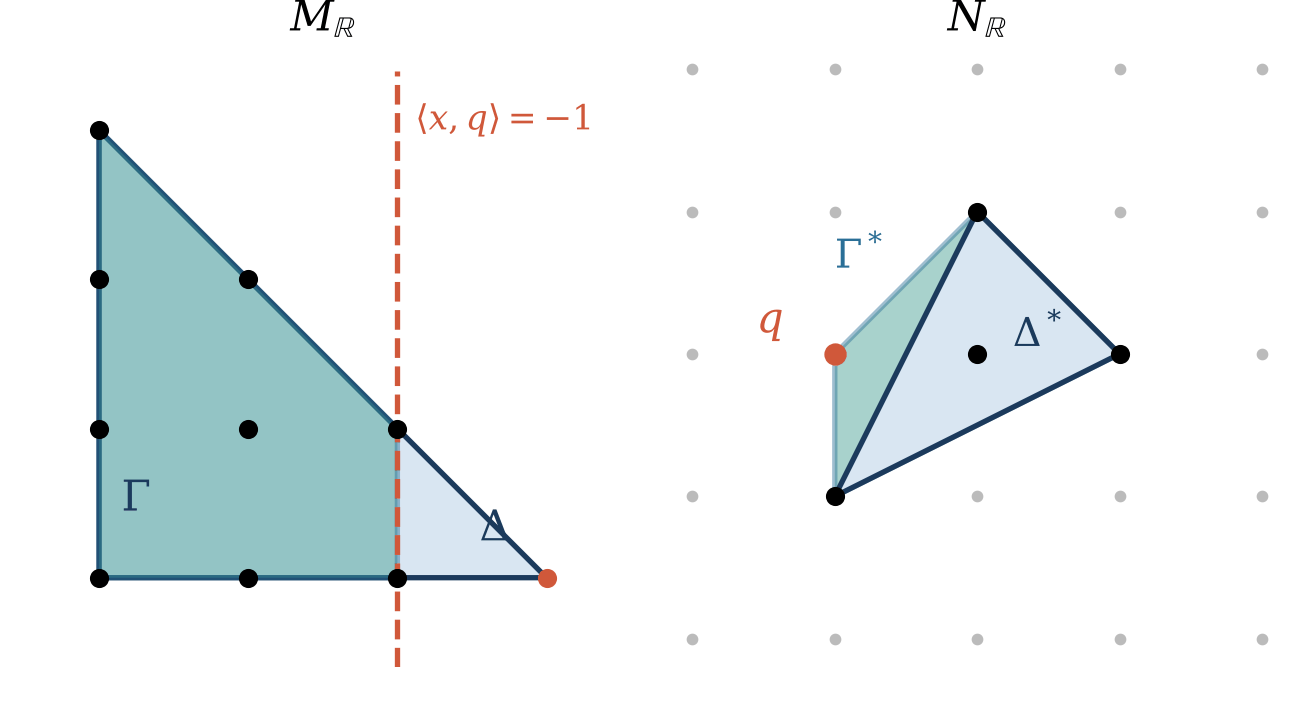
\includegraphics[width=0.72\textwidth]{figures/fig_cut.png}
\caption{A cover as a cut. Left: a reflexive triangle $\Delta$ with ten
lattice points and the cover $\Gamma$ (shaded) obtained by removing the
lattice points with $\ip{x}{q}<-1$. Right: the duals; $\Gamma^*$ is
$\Delta^*$ with the new vertex $q$, and the added piece is the pyramid of
Proposition~\ref{prop:cuts}(c) over the facet of $\Delta^*$ visible from
$q$.}\label{fig:cut}
\end{figure}

Listing all covers is still expensive for the largest polytopes. To walk
down from a polytope it is enough to certify one cover at a time, and for
that the following lemma needs only the dual lattice points of the
candidate.

\begin{lemma}[Climbing lemma]\label{lem:climb}
Let $\Gamma\subsetneq\Delta$ be reflexive. If $H_{q'}=\Gamma$ for
every lattice point $q'$ of $\Gamma^*$ outside $\Delta^*$, then $\Gamma$ is
a cover of $\Delta$.
\end{lemma}

\begin{proof}
Suppose $\Gamma\subsetneq\Gamma'\subsetneq\Delta$ with $\Gamma'$ reflexive.
Then $\Delta^*\subsetneq\Gamma'^*\subsetneq\Gamma^*$, so the lattice
polytope $\Gamma'^*$ has a vertex $q'\notin\Delta^*$, and $q'$ is a lattice
point of $\Gamma'^*$ and of $\Gamma^*$. The cut lemma, applied to
$\Gamma'\subseteq\Delta$ and $q'$, gives $\Gamma'\subseteq H_{q'}=\Gamma$,
a contradiction.
\end{proof}

The lemma turns into a procedure. Start from a cut $q$ with $H_q$
reflexive. For each lattice point $q'$ of $\Gamma^*$ outside $\Delta^*$,
the polytope $H_{q'}$ contains $\Gamma$ by the cut lemma; if it is
reflexive and larger, replace $\Gamma$ by it and start again. Since the
polytopes grow inside $\Delta$, this stops. When it stops with
$H_{q'}=\Gamma$ for every such $q'$, the lemma certifies $\Gamma$ as a
cover; every step of the descent of Section~\ref{sec:four} that is
attributed to the climbing lemma was certified in this way. Choosing the first cut so that $\Gamma$ is small
gives descents that lose many points per step, which is how the descent
of Section~\ref{sec:four} was found.

\section{Dimensions two and three}\label{sec:low}

In dimension two covers are simple.

\begin{proposition}\label{prop:twod}
If $\Gamma$ is a cover of a reflexive polygon $\Delta$, then
$|\Gamma|=|\Delta|-1$. Every r-minimal polygon $E\subseteq\Delta$ is the
last member of some reflexive descent of $\Delta$, and the transition depth
of a reflexive polygon is $\delta(\Delta)=|\Delta|-m(\Delta)$, where
$m(\Delta)$ is the largest number of lattice points of an r-minimal polygon
inside $\Delta$.
\end{proposition}

\begin{proof}
A lattice polygon with exactly one interior lattice point is
reflexive~\cite{PRV00}. Let $\Gamma\subsetneq\Delta$ be reflexive. Some
vertex $v$ of $\Delta$ is not in $\Gamma$, and
$\Delta'=\conv\bigl((\Delta\cap M)\setminus\{v\}\bigr)$ contains $\Gamma$,
hence the origin in its interior, and has no other interior lattice point;
so $\Delta'$ is reflexive, contains $\Gamma$, and has exactly
$|\Delta|-1$ lattice points, since a vertex is not in the hull of the
other lattice points. If $\Gamma$ is a cover, then $\Gamma=\Delta'$.

The same argument, applied to any reflexive $P$ with $E\subsetneq
P\subseteq\Delta$ and a vertex of $P$ outside $E$, gives a cover of $P$
that still contains $E$, so repeating it gives a descent of $\Delta$ that
ends at $E$, of length $|\Delta|-|E|$. Every descent loses one point per
step and ends at an r-minimal polygon, which gives the formula.
\end{proof}

\begin{proof}[Proof of Theorem~\ref{thm:C} in dimension two]
There are sixteen reflexive polygons, listed in Appendix~\ref{app:twod}
with their covers; three are r-minimal, the square
$\conv(\pm e_1,\pm e_2)$ and the triangle with vertices $(1,0)$, $(0,1)$,
$(-2,-1)$ with five lattice points each, and the triangle with vertices
$(1,0)$, $(0,1)$, $(-1,-1)$ with four. Every polygon with at least six
lattice points contains one of the two r-minimal polygons with five points
(the table names one), so by Proposition~\ref{prop:twod} its transition
depth is $|\Delta|-5$. The largest polygon is the triangle
$\conv\{(-1,-1),(2,-1),(-1,2)\}$ with ten lattice points; it contains the
square, so its depth is $5$, and every other polygon has at most nine
points and depth at most $4$. Hence $D_2=5$, attained only by this
triangle. It also contains the triangle with four points, so its longest
descent has $6$ steps.
\end{proof}

Fig.~\ref{fig:hasse2} shows the whole order. The argument uses only that
in the plane one interior point forces reflexivity; that fails from
dimension three on, and there covers can drop many points at once.

\begin{figure}[t]
\centering
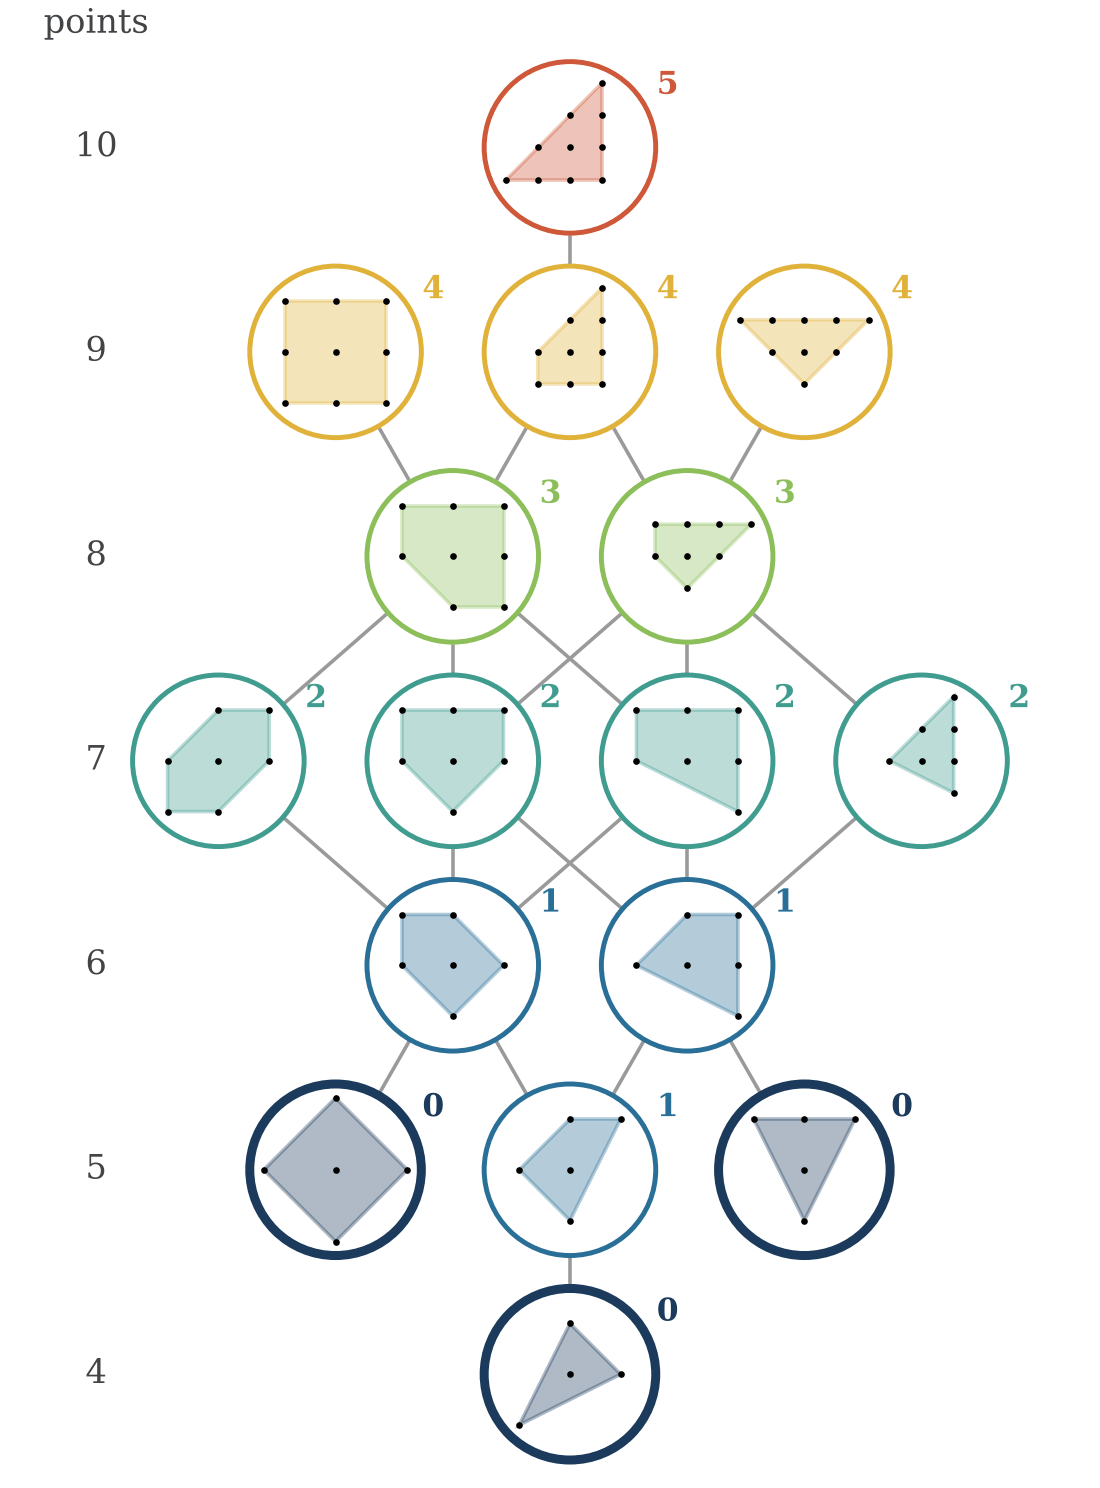
\includegraphics[width=0.62\textwidth]{figures/fig_hasse2.png}
\caption{The sixteen reflexive polygons ordered by inclusion, by number of
lattice points; edges are covers and the number beside each polygon is its
transition depth. The three r-minimal polygons are drawn with thick
circles.}\label{fig:hasse2}
\end{figure}

In dimension three we computed the covers of all $4{,}319$ reflexive
polytopes in two independent ways. The first enumerates, for each
polytope, all lattice polytopes obtained by repeatedly removing a vertex
and taking the convex hull of the remaining lattice points, as long as the
origin stays inside; up to unimodular equivalence this gives $665{,}599$
polytopes, among them every reflexive subpolytope, and the covers are read
off as maximal elements. The second uses Corollary~\ref{cor:covers} with
$V_3=72$. The two agree on all $4{,}303$ polytopes that are not r-minimal,
and give $21{,}841$ covers in all.

\begin{proof}[Proof of Theorem~\ref{thm:C} in dimension three]
With the cover relation known, transition depths follow by induction on
the number of lattice points: $\delta(\Delta)=0$ if $\Delta$ has no cover
and $\delta(\Delta)=1+\min\delta(\Gamma)$ over its covers otherwise. The
maximum is $11$, attained by exactly two polytopes. The first has $35$
lattice points and vertices
\begin{gather*}
(1,0,0),\ (1,2,0),\ (-3,-2,0),\\
(1,2,4),\ (-3,-2,-4),
\end{gather*}
and the second has $31$ lattice points and vertices
\begin{gather*}
(1,0,0),\ (0,1,0),\ (1,0,2),\\
(1,-4,-2),\ (-2,3,2),\ (-2,-1,-2).
\end{gather*} Neither is contained in a larger
reflexive polytope, and both have longest descents of $23$ steps.
\end{proof}

The distribution of depths in dimension three is shown in
Fig.~\ref{fig:depth3}. The longest descent of any three-polytope has $28$
steps, against a simple counting bound of $33$, and sixteen polytopes are
r-minimal. Shortest and longest descents differ a great deal. The mean
transition depth is $5.67$, while the mean length of a longest descent is
$10.23$, so a well-chosen descent is on average a little more than half as
long as a badly chosen one.

\begin{figure}[t]
\centering
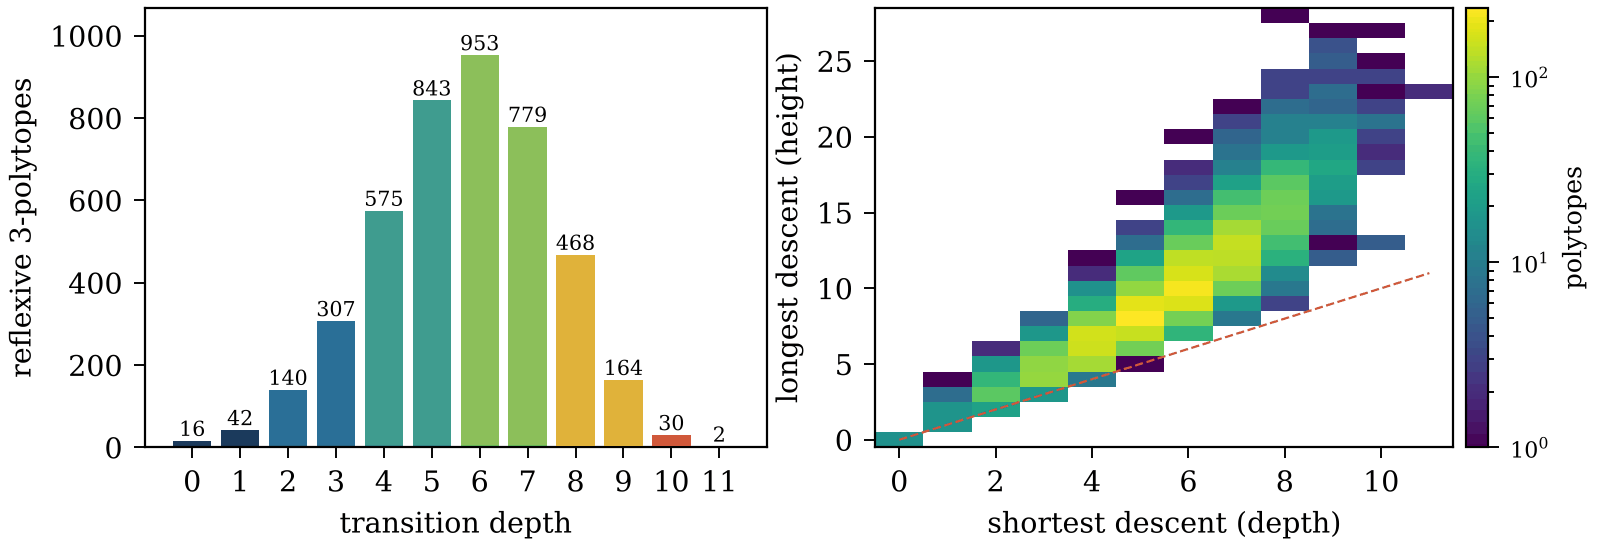
\includegraphics[width=\textwidth]{figures/fig_depth3.png}
\caption{Reflexive three-polytopes. Left: the number of polytopes with
each transition depth. Right: transition depth against the length of the
longest descent, with the diagonal dashed.}\label{fig:depth3}
\end{figure}

\section{Dimension four}\label{sec:four}

\begin{table}[t]
\caption{The sixteen reflexive polygons. Here $|\Delta|$ is the number of
lattice points, $c$ the number of covers, $\delta$ the transition depth and
$h$ the length of a longest descent; the last column gives an r-minimal
subpolygon with five lattice points. The three r-minimal polygons are the
last two rows with five points and the row with four.}\label{tab:twod}
\centering
\begin{adjustbox}{max width=\linewidth}\begin{tabular}{llrrrl}
\toprule
vertices of $\Delta$ & $|\Delta|$ & $c$ & $\delta$ & $h$ & five-point r-minimal polygon inside $\Delta$\\
\midrule
$(-2,-3)$, $(1,0)$, $(1,3)$ & $10$ & $1$ & $5$ & $6$ & $(-1,-2)$, $(0,1)$, $(1,0)$\\
$(-2,1)$, $(0,1)$, $(1,-2)$, $(1,0)$ & $9$ & $2$ & $4$ & $5$ & $(-2,1)$, $(0,1)$, $(1,-1)$\\
$(-1,-2)$, $(-1,0)$, $(1,0)$, $(1,2)$ & $9$ & $1$ & $4$ & $5$ & $(-1,-2)$, $(0,1)$, $(1,0)$\\
$(-3,-2)$, $(1,0)$, $(1,2)$ & $9$ & $1$ & $4$ & $5$ & $(-2,-1)$, $(0,1)$, $(1,0)$\\
$(-1,-2)$, $(-1,1)$, $(0,1)$, $(1,0)$ & $8$ & $3$ & $3$ & $4$ & $(-1,-2)$, $(0,1)$, $(1,0)$\\
$(-1,-1)$, $(-1,1)$, $(0,1)$, $(1,-1)$, $(1,0)$ & $8$ & $3$ & $3$ & $4$ & $(-1,-1)$, $(0,1)$, $(1,-1)$\\
$(-3,-2)$, $(0,1)$, $(1,0)$ & $7$ & $1$ & $2$ & $3$ & $(-2,-1)$, $(0,1)$, $(1,0)$\\
$(-1,-1)$, $(-1,1)$, $(0,-1)$, $(0,1)$, $(1,0)$ & $7$ & $2$ & $2$ & $3$ & $(-1,-1)$, $(-1,1)$, $(1,0)$\\
$(-2,1)$, $(0,-1)$, $(0,1)$, $(1,0)$ & $7$ & $2$ & $2$ & $3$ & $(-2,1)$, $(0,-1)$, $(1,0)$\\
$(-1,0)$, $(-1,1)$, $(0,-1)$, $(0,1)$, $(1,-1)$, $(1,0)$ & $7$ & $1$ & $2$ & $3$ & $(-1,1)$, $(0,-1)$, $(0,1)$, $(1,-1)$\\
$(-1,-1)$, $(-1,1)$, $(0,1)$, $(1,0)$ & $6$ & $2$ & $1$ & $2$ & $(-1,-1)$, $(-1,1)$, $(1,0)$\\
$(-1,0)$, $(0,-1)$, $(0,1)$, $(1,0)$, $(1,1)$ & $6$ & $2$ & $1$ & $2$ & $(-1,0)$, $(0,-1)$, $(0,1)$, $(1,0)$\\
$(-1,0)$, $(0,1)$, $(1,-1)$, $(1,0)$ & $5$ & $1$ & $1$ & $1$ & ---\\
$(-2,-1)$, $(0,1)$, $(1,0)$ & $5$ & $0$ & $0$ & $0$ & ---\\
$(-1,0)$, $(0,-1)$, $(0,1)$, $(1,0)$ & $5$ & $0$ & $0$ & $0$ & ---\\
$(-1,-1)$, $(0,1)$, $(1,0)$ & $4$ & $0$ & $0$ & $0$ & ---\\
\bottomrule
\end{tabular}\end{adjustbox}
\end{table}

\begin{table}[t]
\caption{The reflexive descent $\Gamma_0=\Dbig\supsetneq\Gamma_1\supsetneq
\cdots\supsetneq\Gamma_{38}$: lattice points of $\Gamma_i$ and of
$\Gamma_i^*$, and vertices of $\Gamma_i$.}\label{tab:chain}
\centering
\begin{adjustbox}{max width=\linewidth}\begin{tabular}{lrrrrrrrrrrrrr}
\toprule
$i$ & $0$ & $1$ & $2$ & $3$ & $4$ & $5$ & $6$ & $7$ & $8$ & $9$ & $10$ & $11$ & $12$\\
\midrule
$|\Gamma_i|$ & $680$ & $422$ & $236$ & $207$ & $137$ & $122$ & $103$ & $78$ & $57$ & $44$ & $37$ & $36$ & $35$\\
$|\Gamma_i^*|$ & $26$ & $27$ & $28$ & $29$ & $30$ & $32$ & $33$ & $34$ & $35$ & $36$ & $37$ & $38$ & $39$\\
vert. & $5$ & $7$ & $7$ & $9$ & $11$ & $9$ & $7$ & $9$ & $7$ & $7$ & $5$ & $6$ & $6$\\
 &  &  &  &  &  &  &  &  &  &  &  &  & \\
$i$ & $13$ & $14$ & $15$ & $16$ & $17$ & $18$ & $19$ & $20$ & $21$ & $22$ & $23$ & $24$ & $25$\\
$|\Gamma_i|$ & $34$ & $33$ & $32$ & $31$ & $30$ & $29$ & $28$ & $27$ & $26$ & $25$ & $24$ & $23$ & $22$\\
$|\Gamma_i^*|$ & $40$ & $42$ & $44$ & $46$ & $48$ & $51$ & $54$ & $58$ & $62$ & $66$ & $70$ & $80$ & $86$\\
vert. & $6$ & $7$ & $7$ & $7$ & $7$ & $7$ & $7$ & $7$ & $7$ & $7$ & $7$ & $8$ & $8$\\
 &  &  &  &  &  &  &  &  &  &  &  &  & \\
$i$ & $26$ & $27$ & $28$ & $29$ & $30$ & $31$ & $32$ & $33$ & $34$ & $35$ & $36$ & $37$ & $38$\\
$|\Gamma_i|$ & $21$ & $20$ & $19$ & $18$ & $17$ & $16$ & $15$ & $14$ & $13$ & $12$ & $11$ & $10$ & $9$\\
$|\Gamma_i^*|$ & $88$ & $92$ & $104$ & $116$ & $128$ & $140$ & $152$ & $164$ & $179$ & $188$ & $196$ & $200$ & $201$\\
vert. & $7$ & $7$ & $8$ & $8$ & $8$ & $8$ & $8$ & $7$ & $7$ & $7$ & $7$ & $6$ & $5$\\
\bottomrule
\end{tabular}\end{adjustbox}
\end{table}

The largest reflexive four-polytope is the simplex
\begin{multline*}
\Dbig=\conv\{(-1,-1,-1,-1),\,(83,-1,-1,-1),\\
(-1,6,-1,-1),\,(-1,-1,2,-1),\,(-1,-1,-1,1)\}.
\end{multline*}
Its lattice points are the exponents of the monomials of degree $84$ in
the weighted projective space $\mathbb{P}(1,1,12,28,42)$, shifted by the
interior point $(1,1,1,1)$, so it has $680$ lattice points. The dual
simplex has vertices $e_1,e_2,e_3,e_4$ and $(-1,-12,-28,-42)$, $26$
lattice points and normalised volume $1+1+12+28+42=84$, and $\Dbig$ has
normalised volume $3528=2\cdot42^2$, the largest possible~\cite{BKN22}.
The weights divided by their sum are $\tfrac12,\tfrac13,\tfrac17,
\tfrac1{84},\tfrac1{84}$, which add up to $1$ because
$\tfrac12+\tfrac13+\tfrac17+\tfrac1{42}=1$; here $2,3,7,43$ are the first
terms of Sylvester's sequence and $42=43-1$. The hypersurfaces have Hodge numbers
$(h^{1,1},h^{2,1})=(11,491)$, and their mirror has the largest $h^{1,1}$ in
the list.

Because $\Dbig$ is a simplex, no proper subset of its vertices spans a
polytope with the origin inside, so vertex deletion cannot even start
(Proposition~\ref{prop:vertexdeletion}). Reflexive descent works
(Fig.~\ref{fig:chain680}). Ten steps of the climbing procedure of
Section~\ref{sec:cuts} take the number of lattice points through
\[
680,\ 422,\ 236,\ 207,\ 137,\ 122,\ 103,\ 78,\ 57,\ 44,\ 37,
\]
each step certified as a cover by Lemma~\ref{lem:climb}. From $37$ points
on, all covers were computed by Corollary~\ref{cor:covers}; each step
removes one point, and after $38$ steps the descent reaches a simplex with
nine lattice points and vertices
\begin{gather*}
(-1,-1,-1,1),\ (-1,-1,2,-1),\ (-1,0,1,-1),\\
(-1,6,-1,-1),\ (1,0,0,0),
\end{gather*}
which has no reflexive subpolytope and is itself minimal. The dual counts
rise from $26$ to $201$ along the way. Appendix~\ref{app:chain} lists the
whole descent.

\begin{figure}[t]
\centering
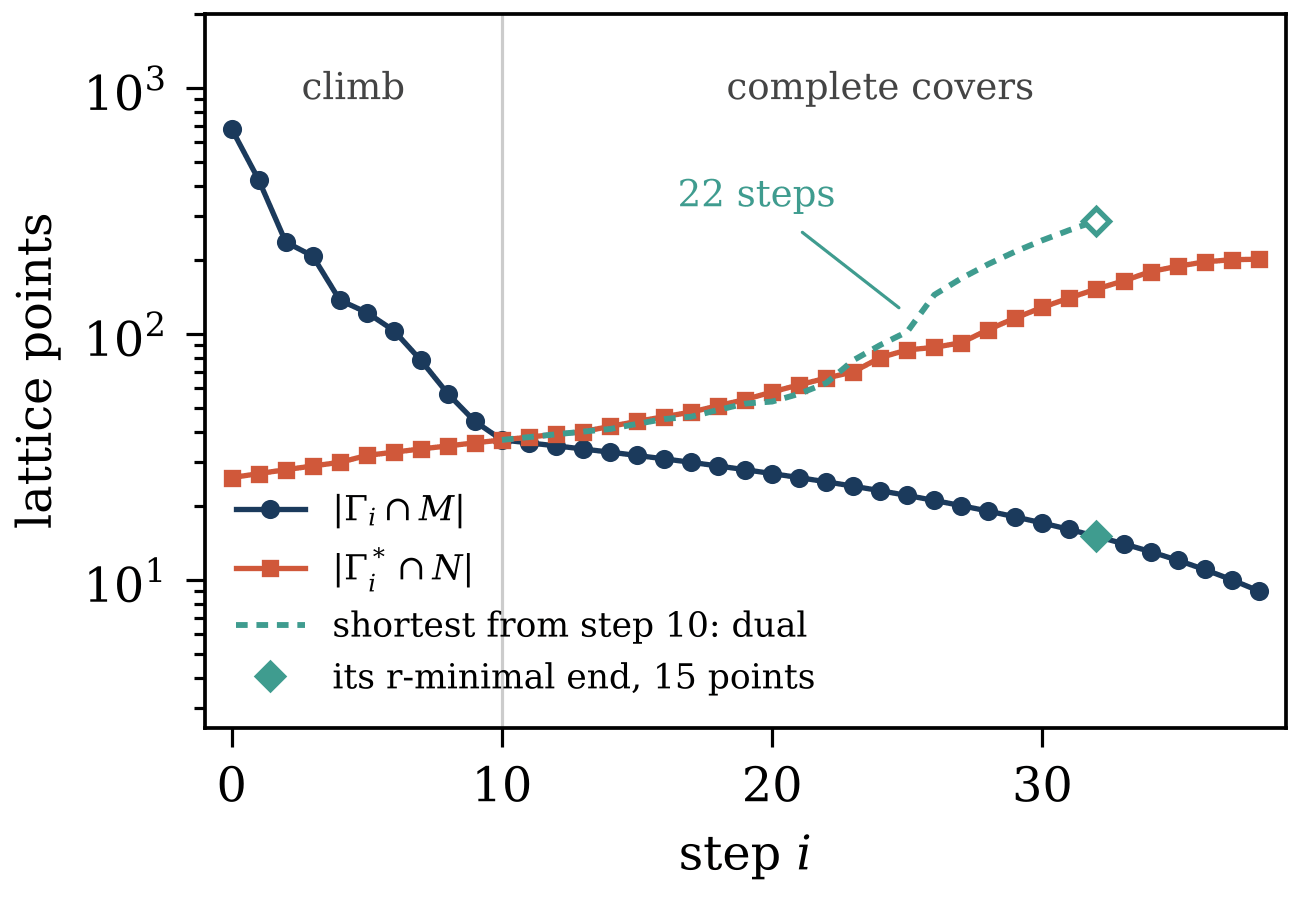
\includegraphics[width=0.72\textwidth]{figures/fig_chain680.png}
\caption{The descent from $\Dbig$: lattice points of $\Gamma_i$ and of its
dual at each step. The first ten covers were certified by the climbing
lemma, the remaining ones by listing all covers. The polytope $\Gamma_{10}$
is the polytope $P_1$ of Section~\ref{ssec:depth22}; a shortest descent of
it has $22$ steps, removes one lattice point at each step like the descent
drawn, and ends at an r-minimal polytope with $15$ lattice points (filled
diamond) whose dual has $288$ (open diamond). The dashed line shows its
dual counts.}
\label{fig:chain680}
\end{figure}

\subsection{A certificate for lower bounds}\label{ssec:certificate}

An upper bound for a transition depth needs one descent, a lower bound a
statement about all of them. The following lemma reduces a lower bound to
a finite object that can be checked one polytope at a time.

\begin{lemma}[Certificate lemma]\label{lem:certificate}
Let $\mathcal{N}$ be a set of reflexive polytopes and
$b\colon\mathcal{N}\to\mathbb{Z}_{\ge0}$ a function such that for every
$\Gamma\in\mathcal{N}$ with $b(\Gamma)>0$ the polytope $\Gamma$ has a
cover, and every cover of $\Gamma$ is unimodularly equivalent to some
$\Gamma'\in\mathcal{N}$ with $b(\Gamma')\ge b(\Gamma)-1$. Then
$\delta(\Gamma)\ge b(\Gamma)$ for every $\Gamma\in\mathcal{N}$.
\end{lemma}

\begin{proof}
A unimodular map fixes the lattice and the origin and preserves inclusion,
so it carries covers to covers and r-minimal polytopes to r-minimal ones;
hence $\delta$ is constant on classes of unimodularly equivalent
polytopes. We use induction on $|\Gamma|$. If $b(\Gamma)=0$ there is
nothing to prove. Otherwise $\Gamma$ has a cover, so it contains a
reflexive polytope other than itself and is not r-minimal, and every
descent $\Gamma=\Gamma_0\supsetneq\Gamma_1\supsetneq\cdots\supsetneq
\Gamma_k$ has $k\ge1$. Its first step $\Gamma_1$ is a cover of $\Gamma$,
so it is equivalent to some $\Gamma'\in\mathcal{N}$ with $b(\Gamma')\ge
b(\Gamma)-1$, and $|\Gamma'|=|\Gamma_1|<|\Gamma|$ by
Lemma~\ref{lem:basic}(i). The chain $\Gamma_1\supsetneq\cdots\supsetneq
\Gamma_k$ is a descent of $\Gamma_1$, so the induction hypothesis gives
$k-1\ge\delta(\Gamma_1)=\delta(\Gamma')\ge b(\Gamma')\ge b(\Gamma)-1$, and
$k\ge b(\Gamma)$.
\end{proof}

The lemma asks for a complete list of covers only at the polytopes with
positive bound, and Corollary~\ref{cor:covers} provides such lists. The
polytopes need not be the same as those of any particular descent, and the
bounds need not be exact depths. A certificate is produced by a bounded
search: to show $\delta(\Gamma)>\ell$ it lists the covers of $\Gamma$ and
shows $\delta(\Gamma')>\ell-1$ for each of them, identifying unimodularly
equivalent polytopes by their normal forms and keeping every bound it has
proved, so that a polytope reached along many paths is examined
once.\footnote{The search is a depth-first search with a memory of exact
depths and of lower bounds. For a bound $\ell$ it tries the covers of
$\Gamma$ in the order of their known depths, smallest first, and stops as
soon as one of them has depth at most $\ell-1$; if none has, the bound
$\delta(\Gamma)\ge\ell+1$ is recorded. Repeating with $\ell=0,1,2,\dots$
gives the exact depth, and the recorded bounds of all polytopes that were
reached form a function $b$ as in Lemma~\ref{lem:certificate}. Exact depths
found on the way are recorded as well; they give the descents that prove the
matching upper bounds.} The certificate is then checked by a program that
does not repeat the search: it verifies the hypothesis of the lemma
polytope by polytope and recomputes the lists of covers.

\subsection{Two polytopes of depth twenty-two}\label{ssec:depth22}
\enlargethispage{4pt}

Let $e_1,\dots,e_4$ be the standard basis of $M=\mathbb{Z}^4$, put
$u=(-4,-2,-1,0)$, and let
\begin{align*}
P_1&=\conv\{e_1,\,e_2,\,e_3,\,u+8e_4,\,u-8e_4\},\\
P_2&=\conv\{e_1,\,e_2,\,e_3,\,u,\,u+8e_4,\,e_3-8e_4\}.
\end{align*}
Both polytopes contain $Q\times\{0\}$, where the tetrahedron
$Q=\conv\{e_1,e_2,e_3,(-4,-2,-1)\}$ lies in $\mathbb{R}^3$ with the
lattice $\mathbb{Z}^3$, and both are bipyramids over it with apexes
at height $\pm8$: $P_1$ is the convex hull of $Q\times\{0\}$ and the two
points $((-4,-2,-1),\pm8)$, and $P_2$ that of $Q\times\{0\}$ and the points
$((-4,-2,-1),8)$ and $(e_3,-8)$. The tetrahedron $Q$ is reflexive, it is the
simplex of the weights $(4,2,1,1)$ because $4e_1+2e_2+e_3+(-4,-2,-1)=0$, and
it has the seven lattice points
\[
e_1,\ e_2,\ e_3,\ (-4,-2,-1),\ (-2,-1,0),\ (-1,0,0),\ 0.
\]
It contains no reflexive polytope other than itself, so it is r-minimal
and its transition depth in dimension three is $0$.

The polytope $P_1$ is a simplex, and
$8e_1+4e_2+2e_3+(u+8e_4)+(u-8e_4)=0$, so it is the simplex of the weights
$(8,4,2,1,1)$. Its lattice points lie on vertical lines over the lattice
points of $Q$. A point $(x,t)$ with $x\in Q$ lies in $P_1$ exactly when
$|t|\le8\lambda(x)$, where $\lambda(x)$ is the barycentric coordinate of
$x$ in $Q$ at the vertex $(-4,-2,-1)$; indeed, writing
$(x,t)=\mu_1e_1+\mu_2e_2+\mu_3e_3+\alpha(u+8e_4)+\beta(u-8e_4)$ with
nonnegative coefficients of sum $1$ gives $\alpha+\beta=\lambda(x)$ and
$t=8(\alpha-\beta)$. The barycentric coordinates of the four lattice
points $(-4,-2,-1)$, $(-2,-1,0)=\tfrac12(-4,-2,-1)+\tfrac12e_3$,
$(-1,0,0)=\tfrac14(-4,-2,-1)+\tfrac12e_2+\tfrac14e_3$ and
$0=\tfrac18(-4,-2,-1)+\tfrac12e_1+\tfrac14e_2+\tfrac18e_3$ at that vertex
are $1,\tfrac12,\tfrac14,\tfrac18$, so the lines over them carry $17$,
$9$, $5$ and $3$ lattice points, and the three points $e_1,e_2,e_3$ carry
one each (Fig.~\ref{fig:depth22}(a)). Hence
\[
|P_1|=17+9+5+3+3=37.
\]
The dual simplex $P_1^*$ has the vertices $(-1,-1,-1,\pm1)$,
$(-1,-1,7,0)$, $(-1,3,-1,0)$ and $(1,-1,-1,0)$, read off from the five
facets of $P_1$, and it also has $37$ lattice points. The polytope $P_2$ has
six vertices, and $|P_2|=|P_2^*|=37$. For both polytopes the Calabi--Yau
hypersurfaces have Hodge numbers $(h^{1,1},h^{2,1})=(34,34)$.

\begin{figure}[t]
\centering
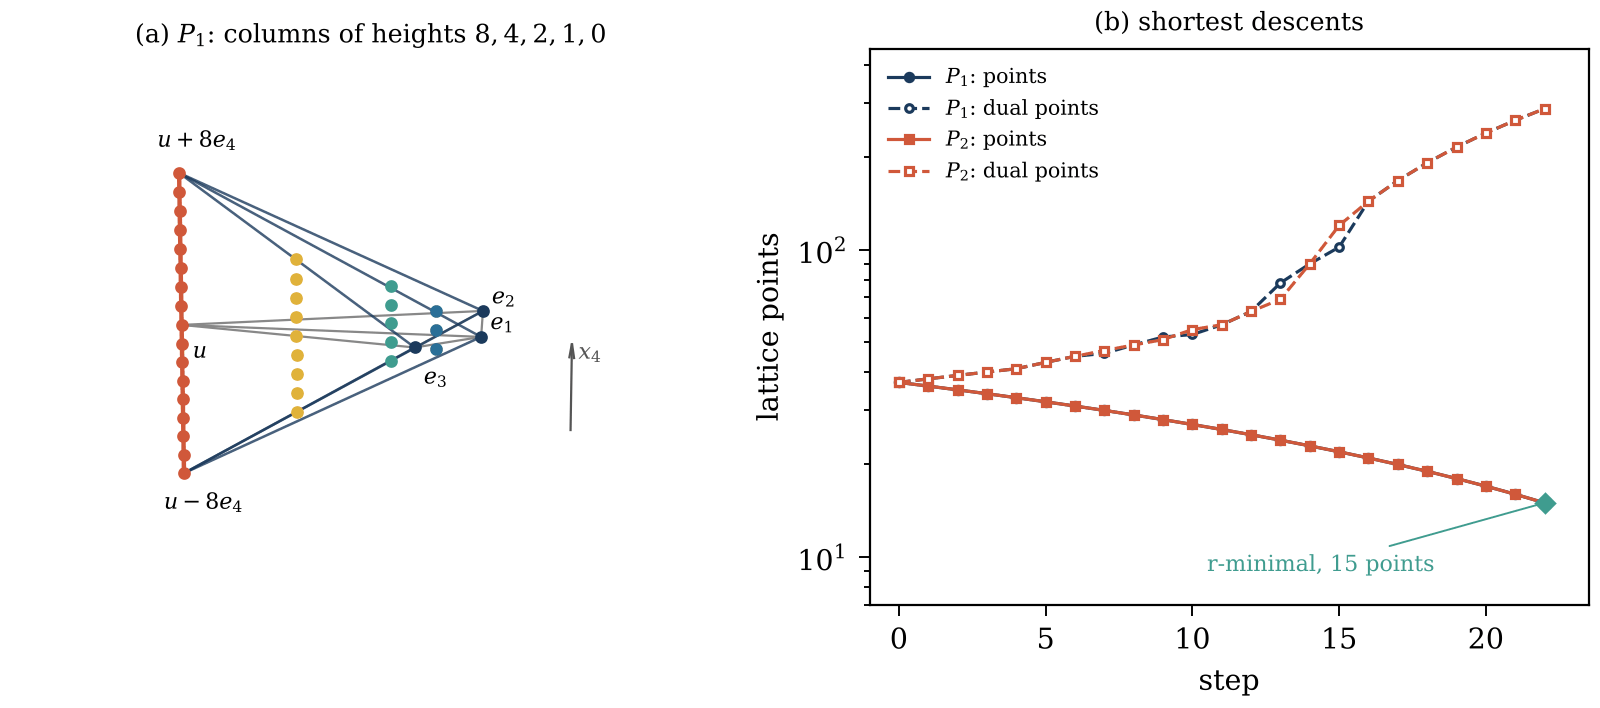
\includegraphics[width=\textwidth]{figures/fig_depth22.png}
\caption{(a) The polytope $P_1$ as a bipyramid over the tetrahedron
$Q\times\{0\}$ (grey edges), with the fourth coordinate vertical. Its $37$
lattice points lie on vertical lines over the seven lattice points of $Q$,
with $17$, $9$, $5$ and $3$ points over $(-4,-2,-1)$, $(-2,-1,0)$,
$(-1,0,0)$ and $0$ and one point at each of $e_1,e_2,e_3$; the half-lengths
$8,4,2,1,0$ of these lines are $8$ times the barycentric coordinate at the
vertex $(-4,-2,-1)$ of $Q$. (b) Lattice points (solid) and dual lattice
points (dashed) along shortest descents of $P_1$ and $P_2$. Each step
removes one lattice point, and both descents end at the same r-minimal
polytope, with $15$ lattice points and $288$ dual lattice points
(diamond).}\label{fig:depth22}
\end{figure}

The two polytopes were found by a search over skew bipyramids
$\conv(Q'\times\{0\}\cup\{(a,k),(b,-k)\})$ over three-dimensional
reflexive polytopes $Q'$, with $a,b$ lattice points of $Q'$ and $k\ge1$,
ranked by the length of a descent found greedily with the cuts of
Section~\ref{sec:cuts}; the exact depths of the highest ranked were then
computed with complete lists of covers.\footnote{The search was organised
on the Anaxia engine of the BLLM programme~\cite{Ana26,BB26}, release
3.0.5, its whole record was rerun on release 3.1.1, and it is kept in release 3.2.1. Anaxia runs a failure-driven loop: each strategy for a target is a
list of checks, a computation or a proof with a named source, a failed
check is recorded together with the change of strategy it forces, all
checks are rerun from the archived data, and the label of a target (open,
candidate, proved) is computed from the record, never assigned by hand.
For the upper bound of Theorem~\ref{thm:B} its record shows the first two
strategies failing: descent by deleting one vertex at a time fails on $7$
of $400$ sampled three-dimensional polytopes, which have no reflexive
vertex deletion, and cuts at dual lattice points of gauge two miss covers
on $73$ of the $400$; the change forced by the second failure was the
complete set of cuts of Corollary~\ref{cor:covers}, which agrees with the
vertex-deletion order on all of them. For the sharp form of
Conjecture~\ref{conj:depth} the first strategy, a sweep of the whole list,
failed on cost, since $162{,}328{,}050$ polytopes have
$\min(|\Delta|-6,680-|\Delta^*|)>40$; the second and third gave the descent
of $\Dbig$ with exact depths of small polytopes along it; the fourth was
the search over skew bipyramids that produced $P_1$ and $P_2$, with the
certificate of Proposition~\ref{prop:depth22} and the identification of
Proposition~\ref{prop:gamma10} as its checks. Its check that the sharp
constant is determined fails, and that target stays open. The engine
organises and reruns the computations; every statement of this section is
proved in the text, and the certificate is checked by the programs of
Appendix~\ref{app:checks}, which do not use the engine.}

\begin{proposition}\label{prop:depth22}
$\delta(P_1)=\delta(P_2)=22$.
\end{proposition}

\begin{proof}
For the upper bound, each of $P_1$ and $P_2$ has a descent of $22$ steps,
each step a cover by Corollary~\ref{cor:covers}. Both remove one lattice
point at each step, so the numbers of lattice points run through
$37,36,\dots,15$, while the dual counts rise from $37$ to $288$
(Fig.~\ref{fig:depth22}(b)). Both end at the same polytope, with vertices
\[
(-4,-2,-1,7),\ (-2,-1,0,-1),\ (-2,-1,0,4),\ e_1,\ e_2,\ e_3,
\]
$15$ lattice points and no cover.

For the lower bound we apply Lemma~\ref{lem:certificate} to a set
$\mathcal{N}$ of $5{,}592$ polytopes containing $P_1$ and $P_2$, with
$b(P_1)=b(P_2)=22$. Of these, $5{,}250$ have positive bound; for each of
them the set $\mathcal{N}$ contains a representative of every cover, given
by the complete list of Corollary~\ref{cor:covers}, $23{,}646$ covers in
all, and each cover has bound at least one less. The lemma gives
$\delta(P_1),\delta(P_2)\ge22$.
\end{proof}

The polytopes of the certificate have between $14$ and $37$ lattice
points; the most frequent sizes are $17$ to $20$ points, with between
$472$ and $494$ polytopes each, and only $61$ polytopes have more than
$31$ points.

\begin{proposition}\label{prop:gamma10}
The matrix
\[
G=\begin{pmatrix}-1&-1&-1&-1\\-1&-1&6&0\\-1&2&-1&0\\1&-1&-1&0\end{pmatrix}
\]
is unimodular, and $x\mapsto Gx$ carries $P_1$ onto the polytope
$\Gamma_{10}$ of the descent of $\Dbig$ in Table~\ref{tab:chain}. Hence
$\delta(\Gamma_{10})=22$ and $\delta(\Dbig)\le32$.
\end{proposition}

\begin{proof}
The matrix
\[
H=\begin{pmatrix}0&3&7&11\\0&2&5&7\\0&1&2&3\\-1&-6&-14&-21\end{pmatrix}
\]
is integral and $GH=1$, so $G$ is unimodular. The map sends $e_1$, $e_2$,
$e_3$, $u+8e_4$ and $u-8e_4$ to
\begin{gather*}
(-1,-1,-1,1),\ (-1,-1,2,-1),\ (-1,6,-1,-1),\\
(-1,0,1,-1),\ (15,0,1,-1),
\end{gather*}
which are the five vertices of the simplex $\Gamma_{10}$. Since
$\Gamma_{10}$ is reached from $\Dbig$ by ten covers,
$\delta(\Dbig)\le10+\delta(\Gamma_{10})=10+22$.
\end{proof}

Three of the vertices of $\Gamma_{10}$ are vertices of $\Dbig$, and the
other two lie on its facet $x_4=-1$. One step higher the same search gives
a descent of $22$ steps from $\Gamma_9$, which has $44$ lattice points: it
removes one or two points at a time and ends at an r-minimal polytope with
$19$ lattice points. Hence $\delta(\Dbig)\le9+22=\DUB$.

\begin{proof}[Proof of Theorem~\ref{thm:D}]
Proposition~\ref{prop:depth22} gives $\delta(P_1)=\delta(P_2)=\LB$, so
$D_4\ge\LB$, and Proposition~\ref{prop:gamma10} identifies $P_1$ with
$\Gamma_{10}$. The nine covers from $\Dbig$ to $\Gamma_9$ in
Table~\ref{tab:chain}, each certified by the climbing lemma,
followed by the descent of $22$ steps from $\Gamma_9$, form a descent of
$\Dbig$ of length $\DUB$. Finally $D_4\le\UB$ by Theorem~\ref{thm:B}.
\end{proof}

Smaller polytopes along the descent of $\Dbig$ have smaller depth: the
same search gives $\delta(\Gamma_{27})=9$ for the polytope with twenty
lattice points and $\delta(\Gamma_{32})=4$ for the one with fifteen, and
among the four-polytopes with at most eleven lattice points the largest
transition depth is $5$.

\section{Free sums, exact families and growth with dimension}\label{sec:freesums}
The question of a lower bound increasing with the dimension has a
constructive answer. The operation is the free sum in a \emph{direct-sum
lattice}. Its polarity and lattice-point behavior are standard; related
enumerative identities are studied by Braun~\cite{Braun06}. We give the
arguments needed here, including the order isomorphism and the consequences
for saturated descents. No classification or four-dimensional census is
used in the proofs of this section's structural theorems.

Let $M,N$ be lattices, and let $P\subset M_\R$ and $Q\subset N_\R$
be full-dimensional reflexive polytopes. Define
\[
 P\oplus Q=\conv\bigl((P\times\{0\})\cup(\{0\}\times Q)\bigr)
 \subset (M\oplus N)_\R.
\]
The direct-sum lattice is essential: we do not pass to an overlattice.

\begin{lemma}[Lattice points of a free sum]\label{lem:fs-points}
The free sum is reflexive and
\[
 (P\oplus Q)^*=P^*\times Q^*,\qquad
 (P\oplus Q)\cap(M\oplus N)
 =((P\cap M)\times\{0\})\cup(\{0\}\times(Q\cap N)).
\]
In particular $|P\oplus Q|=|P|+|Q|-1$.
\end{lemma}
\begin{proof}
A linear functional $(u,v)$ is at least $-1$ on both factor polytopes
exactly when $u\in P^*$ and $v\in Q^*$, proving the polar formula.
The vertices of this product are pairs of lattice vertices, so the
free sum is reflexive.

For a polytope $P$ containing zero in its interior, write
$g_P(x)=\inf\{t\ge0:x\in tP\}$ for its gauge. From the definition of
the free sum,
\begin{equation}\label{eq:fs-gauge}
 (x,y)\in P\oplus Q\quad\Longleftrightarrow\quad
 g_P(x)+g_Q(y)\le1.
\end{equation}
Indeed a convex combination of points of the two factor polytopes
gives nonnegative budgets $a,b$ with $a+b=1$, $x\in aP$, $y\in bQ$.
Conversely, if the gauges sum to at most one, enlarge the two budgets
to sum to one and use convexity and $0\in P,Q$.

Zero is the only interior lattice point of a reflexive polytope.
Therefore $g_P(x)\ge1$ for $x\in M\setminus\{0\}$, and similarly for
$Q$. A lattice point with two nonzero components would violate
\eqref{eq:fs-gauge}. The remaining lattice points are exactly those
displayed. The origin belongs to both sets and is counted once.
\end{proof}

\begin{theorem}[Product of reflexive-subpolytope orders]\label{thm:fs-order}
There is an order isomorphism
\[
 R(P)\times R(Q)\longrightarrow R(P\oplus Q),\qquad
 (A,B)\longmapsto A\oplus B.
\]
Every full-dimensional reflexive subpolytope of $P\oplus Q$ has a unique
such factorization in the specified coordinate lattices.
\end{theorem}
\begin{proof}
Let $C\in R(P\oplus Q)$. Its vertices are lattice points, so
Lemma~\ref{lem:fs-points} places each vertex on a coordinate factor.
Let $A$ and $B$ be the convex hulls of its vertices in those factors.
Both have zero in their interiors, relative to the full factor spaces.
For if, for example, this failed for $A$, a nonzero supporting or
separating linear functional on $M_\R$ would be nonnegative on $A$;
extended by zero on $N_\R$, it would be nonnegative on $C$. This
contradicts $0\in\operatorname{int}C$.
Consequently $C=A\oplus B$, where $A\subseteq P$ and $B\subseteq Q$
are full-dimensional lattice polytopes with zero inside.

Now $C^*=A^*\times B^*$ is a lattice polytope. A product has vertices
exactly the pairs of vertices of its factors; projecting those vertices
shows that $A^*$ and $B^*$ have lattice vertices. Hence $A,B$ are
reflexive. Conversely the free sum of any $A\in R(P)$ and $B\in R(Q)$
is a reflexive subpolytope by Lemma~\ref{lem:fs-points}.

The intersections of $C=A\oplus B$ with the two coordinate subspaces
are precisely $A$ and $B$, since both contain zero. Thus the factors are
unique. These intersections show that inclusion of free sums implies
inclusion in each factor. The reverse implication follows directly
from convex hulls, proving the order isomorphism.
\end{proof}

\begin{corollary}[Covers change one factor]\label{cor:fs-covers}
The lower covers of $A\oplus B$ are exactly
\[
 A'\oplus B\quad(A'\text{ a lower cover of }A),\qquad
 A\oplus B'\quad(B'\text{ a lower cover of }B).
\]
Moreover $A\oplus B$ is r-minimal exactly when both factors are.
\end{corollary}
\begin{proof}
If both factors decreased, changing just one would supply a strict
intermediate reflexive polytope. If one factor decreased by more than a
cover, an intermediate in that factor would do the same. Conversely,
when one factor is fixed and the other changes by a cover, the order
isomorphism leaves no possible intermediate. The statement about
r-minimal elements follows at once.
\end{proof}

Let $h(P)$ be the length of a longest saturated descent from $P$ to an
r-minimal polytope. Both $h(P)$ and $\delta(P)$ exist because $R(P)$ is
finite.

\begin{theorem}[Exact additivity of descent lengths]\label{thm:fs-depth}
One has
\[
 \delta(P\oplus Q)=\delta(P)+\delta(Q),\qquad
 h(P\oplus Q)=h(P)+h(Q).
\]
\end{theorem}
\begin{proof}
Project a saturated descent to the two factor orders and omit repetitions.
By Corollary~\ref{cor:fs-covers} the projections are saturated descents,
and their endpoints are r-minimal. Every step occurs in exactly one
factor, so its length is the sum of the two projected lengths. This
gives the lower bound for $\delta$ and the upper bound for $h$.
Conversely, interleave two shortest descents, respectively two longest
descents, keeping the other factor fixed at each step. Every step is a
cover by the same corollary, and the final free sum is r-minimal.
The two bounds are therefore attained.
\end{proof}

\begin{remark}[Which chains are counted]
We work with actual embedded subpolytopes in the fixed lattice, not with
orbits of chains under automorphisms. A unimodular change of coordinates
preserves the shortest and longest lengths, so the preceding equalities
also compute the transition depth used for the classified polytopes.
The counting statement below retains the embedded, labelled convention.
\end{remark}

For $j\ge0$, let $c_j(P)$ count all saturated descents of length $j$
ending at an r-minimal polytope, and put
\[
 E_P(t)=\sum_{j\ge0}c_j(P)\frac{t^j}{j!}.
\]
This is a polynomial.

\begin{proposition}[Complete descent profile]\label{prop:fs-profile}
The profile satisfies
\[
 c_n(P\oplus Q)=\sum_{a+b=n}\binom{n}{a}c_a(P)c_b(Q),
 \qquad E_{P\oplus Q}(t)=E_P(t)E_Q(t).
\]
\end{proposition}
\begin{proof}
Choose a descent of length $a$ in $P$, one of length $b$ in $Q$, and the
$a$ positions of the first descent among the $a+b$ steps. The cover
description gives a saturated product descent. Its projections recover
both chosen descents and their interleaving uniquely. This is a bijection,
which gives the convolution and then its exponential generating function.
\end{proof}

\subsection{A family with a direct proof and no finite census}
Consider
\[
\begin{gathered}
 B=\conv\{a,b,c,d,e\},\\
 a=(-1,-1),\quad b=(-1,0),\quad c=(0,-1),\\
 d=(0,1),\quad e=(1,0).
\end{gathered}
\]
Its lattice points are these five vertices and zero. For example its
primitive facet inequalities are
\[
 x+y\le1,\quad -x+y\le1,\quad x\ge-1,\quad y\ge-1,\quad x-y\le1.
\]
Thus $B$ is reflexive. Let $A=\conv(a,d,e)$,
$H_b=\conv(a,b,d,e)$, $H_c=\conv(a,c,d,e)$, and
$C=\conv(b,c,d,e)$.

\begin{proposition}[Five-element base order]\label{prop:fs-pentagon}
The embedded reflexive-subpolytope order of $B$ consists of exactly
$A,H_b,H_c,C,B$. The minimal elements are $A,C$. The three lower covers
of $B$ are $H_b,H_c,C$, and each $H_b,H_c$ has the single lower cover
$A$. Consequently
\[
 \delta(B)=1,\quad h(B)=2,\quad c_1(B)=1,\quad c_2(B)=2,
 \qquad E_B(t)=t+t^2.
\]
\end{proposition}
\begin{proof}
Any full-dimensional subpolytope with zero inside must contain $e$,
the only available lattice point with positive first coordinate, and
$d$, the only one with positive second coordinate. If it contains $a$,
the choices are exactly $A,H_b,H_c,B$, according to whether $b,c$ are
included. If it does not contain $a$, it must contain both $b,c$ to
have negative coordinates in both directions; this gives $C$.
The origin cannot be a vertex of a polytope in question, so no other
choice is possible.

All five polytopes have zero in their interiors and are reflexive.
This can be checked from their edges: $A$ has inequalities
$x-2y\le1$, $x+y\le1$, $-2x+y\le1$; $H_b$ has
$x-2y\le1$, $x+y\le1$, $-x+y\le1$, $-x\le1$;
$H_c$ has $-y\le1$, $x-y\le1$, $x+y\le1$, $-2x+y\le1$;
and $C$ has $\pm x\pm y\le1$ with all four choices of signs.
All normals are primitive integral vectors. The inclusion relations
are exactly those stated. In particular
$A$ and $C$ contain no smaller reflexive full-dimensional polytope.
Reading the five-element order proves the depth and profile formulas.
\end{proof}

\begin{figure}[ht]
\centering
\begin{tikzpicture}[scale=.9,every node/.style={font=\small},
 node distance=15mm]
\node (B) at (0,2) {$B\ (6)$};
\node (Hb) at (-2,1) {$H_b\ (5)$};
\node[draw,rounded corners,fill=blue!8,inner sep=4pt] (C) at (0,1) {$C\ (5)$};
\node (Hc) at (2,1) {$H_c\ (5)$};
\node[draw,rounded corners,fill=blue!8,inner sep=4pt] (A) at (0,0) {$A\ (4)$};
\draw (B)--(Hb) (B)--(C) (B)--(Hc) (Hb)--(A) (Hc)--(A);
\end{tikzpicture}
\caption{The complete embedded order for $B$. Parentheses give lattice-point
counts; boxes mark r-minimal polygons. The left and right branches are
different embedded chains even though an automorphism exchanges them.}
\label{fig:fs-base}
\end{figure}

\begin{theorem}[An explicit family of arbitrary depth]\label{thm:fs-family}
For every $r\ge1$, put $B_r=B^{\oplus r}$ in the lattice $\Z^{2r}$.
Then
\[
 |B_r|=5r+1,\quad\delta(B_r)=r,\quad h(B_r)=2r,
 \qquad E_{B_r}(t)=t^r(1+t)^r.
\]
More precisely, for $0\le j\le r$ the number of descents of length
$r+j$ is $(r+j)!\binom rj$, and there are none of other lengths.
In dimension $2r+1$, $B_r\oplus[-1,1]$ has the same depths and profile.
\end{theorem}
\begin{proof}
Apply Lemma~\ref{lem:fs-points} and
Theorem~\ref{thm:fs-depth} repeatedly. The profile follows from
Proposition~\ref{prop:fs-profile} and $E_B(t)=t+t^2$; multiplying the
coefficient of $t^{r+j}$ by $(r+j)!$ gives the stated number.
The interval $[-1,1]$ is the only one-dimensional reflexive polytope,
is r-minimal, and has profile $1$. A free sum with it changes neither
the depths nor the profile.
\end{proof}

This theorem supplies a lower bound growing with dimension and an
unbounded shortest--longest gap by a direct analytic construction.
It uses no census, numerical hull computation, or imported certificate.

\subsection{A stronger small base checked independently}
The triangle
\[
 T=\conv\{(-1,-1),(2,-1),(-1,2)\}
\]
has ten lattice points. Its depths $\delta(T)=5$, $h(T)=6$ also follow
from the planar argument in Section~\ref{sec:low}. For the new profile
calculation and an independent check of this base, we enumerate only
the $2^9=512$ subsets of its nine nonzero lattice points.
Two exact integer implementations are supplied. One takes monotone-chain
convex hulls and closes them in $T\cap\Z^2$; the other uses all supporting
directed pairs and no hull routine. They give the same $79$ embedded
reflexive subpolytopes. Their finite cover order has
\[
 c_5(T)=150,\quad c_6(T)=240,\quad c_j(T)=0\ (j\ne5,6),\qquad
 E_T(t)=\frac54t^5+\frac13t^6.
\]
Appendix~\ref{app:fs-cert} specifies the finite calculation completely.

\begin{corollary}[The triangle family]\label{cor:fs-triangle}
For every $r\ge1$, the explicit polytope $T_r=T^{\oplus r}$ satisfies
\[
 \dim T_r=2r,\quad |T_r|=9r+1,\quad
 \delta(T_r)=5r,\quad h(T_r)=6r,
\]
\[
 E_{T_r}(t)=t^{5r}\left(\frac54+\frac t3\right)^r.
\]
Hence
\[
 c_{5r+j}(T_r)=(5r+j)!\binom rj
                  \left(\frac54\right)^{r-j}\left(\frac13\right)^j
 \quad(0\le j\le r).
\]
The formula counts embedded chains, and its rational expression is an
integer by its counting interpretation. A free sum with $[-1,1]$ gives
the same conclusions in odd dimensions after increasing the dimension by one.
\end{corollary}
\begin{proof}
Use Theorem~\ref{thm:fs-depth}, Proposition~\ref{prop:fs-profile}, and
the exact base profile just specified. No high-dimensional enumeration
is needed.
\end{proof}

\subsection{The extremal depth as a function of dimension}
\begin{theorem}[Superadditivity and an asymptotic limit]\label{thm:fs-growth}
The extremal depths are finite and satisfy
\[
 D_{m+n}\ge D_m+D_n\quad(m,n\ge1),\qquad
 D_d\ge\left\lfloor\frac d2\right\rfloor.
\]
The independent triangle certificate strengthens the second inequality to
\[
 D_d\ge5\left\lfloor\frac d2\right\rfloor.
\]
Moreover the extended limit exists:
\[
 \lim_{d\to\infty}\frac{D_d}{d}
 =\sup_{d\ge1}\frac{D_d}{d}\ \in\ [5/2,\infty].
\]
Using the earlier depth-$22$ result of Theorem~\ref{thm:D} as a
certificate-backed base further gives $D_{4r}\ge22r$ and lower endpoint
$11/2$ for this limit. The last strengthening imports precisely that
earlier finite certificate, not the whole four-dimensional census.
\end{theorem}
\begin{proof}
Proposition~\ref{prop:everydim} bounds all depths for $d\ge4$.
In dimensions two and three finiteness also follows by taking free sums
with intervals to embed a given depth unchanged into dimension four.
The one-dimensional depth is zero. Thus the nonempty set of possible
integer depths in each dimension is bounded and has an attained maximum.
Take polytopes attaining $D_m,D_n$ and apply Theorem~\ref{thm:fs-depth}
to their free sum. This proves superadditivity. The lower bounds follow
from Theorem~\ref{thm:fs-family} and Corollary~\ref{cor:fs-triangle}.

For completeness, set $D_0=0$ for the following arithmetic argument.
For fixed $k\ge1$ write $d=qk+s$, $0\le s<k$. Superadditivity and
nonnegativity give $D_d\ge qD_k+D_s\ge qD_k$. Thus
$\liminf_dD_d/d\ge D_k/k$. Taking the supremum over $k$ and observing
that every $D_d/d$ is at most that supremum proves the equality of
extended limits, including the case of infinite supremum. The base
inequality with $k=2$ gives $5/2$. The same argument with the
certificate-backed $D_4\ge22$ gives $11/2$ when that earlier result is used.
\end{proof}

The analytic family $B_r$ alone settles the existence of a growing
lower bound. The exact growth rate, whether the displayed limit is finite,
and the optimal four-dimensional depth are not determined here.
In particular $\delta(T\oplus T)=10$ is an exact value for that particular
four-polytope, not a replacement for the existing lower bound $D_4\ge22$.

\section{Open questions}\label{sec:open}

The original uniform-existence statement is proved. The exact
four-dimensional maximum is still unknown: the certificate-backed
range is $22\le D_4\le346$ relative to the supplied census. The
upper bound is not claimed sharp, and the heuristic of a few tens
has not been established. Larger lower bounds require complete cover
lists or another argument controlling every descent, rather than one
displayed chain.

The question whether there is a lower bound growing with dimension
now has an affirmative answer by Theorem~\ref{thm:fs-family}.
Theorem~\ref{thm:fs-growth} gives superadditivity and an extended limit
for $D_d/d$, but does not decide whether the limit is finite or give
the optimal rate. The upper bound remains doubly exponential.

The shortest--longest gap is unbounded as dimension varies: $B_r$
and $T_r$ have gap $r$. Its largest value in each fixed dimension is
not determined by that construction. In dimension three the earlier
computation gives a largest gap of $20$, for a $35$-point simplex of
depth $8$ and longest descent $28$ (Fig.~\ref{fig:depth3}).

Whether a polytope attaining $D_4$ must be r-maximal remains open.
The two-dimensional extremizer is the ten-point triangle; both
three-dimensional extremizers are r-maximal. The known depth-$22$
polytope $P_1$ lies inside $\Dbig$ and hence is not r-maximal. The
free-sum theorem describes exact families, without classifying all
extremizers. The unresolved higher-dimensional nonreflexive-cut
behavior in Section~\ref{sec:cuts} is likewise not settled by these
families.

\section*{Data availability}

The original code and data are archived in release 1.2.0 of the repository,
\url{https://github.com/creelie/seed/releases/tag/v1.2.0}~\cite{Repo}. The
archive contains the joint distribution of point counts over the whole
list, the pair bounds, the cover relation in dimensions two and three, the
descent of $\Dbig$ with its certificates, the certificate of
Lemma~\ref{lem:certificate} for $P_1$ and $P_2$, the checks of the cuts formed by
Corollary~\ref{cor:covers} in dimension three and at the certificate polytopes, and independent checks in
C, C++, Python, Julia, Macaulay2, shell and Lean~4. The Kreuzer--Skarke
list was read from its public copy~\cite{HF4D}. The search for long
descents was organised on the Anaxia engine, release 3.0.5, and rechecked
on release 3.1.1; the engine is archived in release 3.2.1~\cite{Ana26} and described in~\cite{BB26}, and its record of strategies,
failed checks and the changes they forced is part of the archive. The original computations and text used Claude (Anthropic).
For this review revision, ChatGPT (OpenAI) assisted with the free-sum
proofs, exact-integer checks and manuscript preparation. The new
\texttt{anc/} directory contains the two base certificates, their
standard-library Python verifier, the interval verifier and its data,
and the current verification report. These additions accompany release v1.3.0 of \url{https://github.com/creelie/seed/releases/tag/v1.3.0}; its version DOI is recorded in the archive receipt. The complete $5{,}592$-node cover reconstruction
from the preceding paper was not rerun in this revision. Its earlier
certificate remains an explicitly imported finite base for the
stronger $22r$ lower bound. The independent pentagon and triangle
families do not require it. The core geometric order isomorphism and depth-additivity results now have Lean proofs, with the precise scope given in Appendix~\ref{app:formal}. The whole manuscript is not formalized.

\section*{Statements and Declarations}

\noindent\textit{Funding.} The author received no funding for this work.

\noindent\textit{Competing interests.} The author declares no competing
interests.

\appendix

\section{The reflexive polygons}\label{app:twod}

Table~\ref{tab:twod} lists the sixteen reflexive polygons by their
vertices, with the number of lattice points, the number of covers, the
transition depth $\delta$ and the length $h$ of a longest descent. For each
polygon with at least six points the last column gives the vertices of an
r-minimal polygon with five lattice points inside it, which is what the
proof of Theorem~\ref{thm:C} needs. Each entry can be checked by hand.

\section{The descent from the largest polytope}\label{app:chain}

Table~\ref{tab:chain} lists the descent of Section~\ref{sec:four}: for each
step $i$ the number of lattice points of $\Gamma_i$ and of its dual and the
number of vertices of $\Gamma_i$. Steps $1$ to $10$ were certified by the
climbing lemma and steps $11$ to $38$ by listing all covers. The lattice
points of every $\Gamma_i$ are in the archive~\cite{Repo}.

\section{How the computations were checked}\label{app:checks}

Every computational statement in the paper was obtained by one method and
confirmed by a second, written independently, where that was practical.

\paragraph*{Point counts.} The joint distribution of $|\Delta|$ and
$|\Delta^*|$ was read from all $473{,}800{,}776$ entries of the
list~\cite{HF4D}. The total, the extreme values $6$ and $680$, and the
single polytope at $(680,26)$ agree with Kreuzer and Skarke~\cite{KS00}.
The pair bound was computed by the recursion of Section~\ref{sec:counting}
and again by a direct quadratic search over all pairs, with the same
result; a separate program checks the bounds $654$ and $348$ and the
counts of Table~\ref{tab:counting}.

\paragraph*{Covers.} In dimension two the sixteen polygons and their
covers were computed from scratch and agree with Table~\ref{tab:twod}. In
dimension three the cover relation obtained by removing lattice points and
the one obtained from Corollary~\ref{cor:covers} agree on every polytope.
Unimodular equivalence was decided with the normal forms of
PALP~\cite{KS04}.

\paragraph*{The simplex $\Dbig$.} Its $680$ lattice points, the $26$ points
of its dual and the volumes $3528$ and $84$ were checked by four separate
programs, and the arithmetic of the weights by a proof assistant. Each
step of the descent in Table~\ref{tab:chain} was certified as a cover, and
the last polytope was checked to have no reflexive proper subpolytope.

\paragraph*{Exact depths.} The values $\delta(\Gamma_{27})=9$ and
$\delta(\Gamma_{32})=4$ come from breadth-first searches through complete
lists of covers, in which unimodularly equivalent polytopes are identified.
The search stops at the first level that contains a polytope without
covers, so it gives the least length of a descent.

\paragraph*{The certificate for $P_1$ and $P_2$.} The archive stores the
$5{,}592$ polytopes of the certificate by their lattice points and PALP
normal forms, the list of covers of each of the $5{,}250$ polytopes with
positive bound ($23{,}646$ covers in all) and of one polytope without
covers, the bound of every polytope, and
the two descents of length $22$. A separate program checks, without PALP,
that every stored point set is the set of lattice points of a reflexive
polytope, that the roots are $P_1$ and $P_2$, that every cover has fewer
lattice points than the polytope it covers, that the bounds satisfy the
hypothesis of Lemma~\ref{lem:certificate} and equal $22$ at the roots,
that both descents end at a polytope without covers, and that the matrix
$G$ of Proposition~\ref{prop:gamma10} is unimodular and carries the
lattice points of $P_1$ onto those of $\Gamma_{10}$. With PALP it
recomputes every normal form and every list of covers by
Corollary~\ref{cor:covers}, and all $5{,}251$ recomputed lists agree with
the stored ones. The descent of length $22$ from $\Gamma_9$ is
stored as a chain of subpolytopes of $\Gamma_9$, and each of its steps is
checked to be a cover in the same way. Lemma~\ref{lem:certificate}, the
point counts along the descents and the arithmetic of $G$ are also
theorems of the Lean file.

\paragraph*{Every dimension.} The step from Blichfeldt's inequality to the
bound of Proposition~\ref{prop:everydim} is a theorem of the Lean file for
every $d$ and every $V$: a chain of point counts that strictly decrease,
stay at least $d+2$ and start at most at $V+d$ has at most $V-2$ steps. A
short program compares the bound with the posets of dimensions two and
three, whose longest chains of covers have $6$ and $28$ steps, and with the
point counts of the list in dimension four.

\section{The exact planar base certificate}\label{app:fs-cert}
We specify the independent finite calculation behind the stronger base.
The nine boundary points of $T$, in the order used by both checkers, are
\[
 (-1,-1),(-1,0),(-1,1),(-1,2),(0,-1),(0,1),(1,-1),(1,0),(2,-1).
\]
A mask $m=\sum_{i=0}^8\varepsilon_i2^i$ selects a subset of these points.
All $512$ masks are examined. A polygon is retained only if zero is
strictly interior and its point set is closed in $T\cap\Z^2$.
Reflexivity is checked directly from primitive edge distances, not from
a floating-point hull calculation.

\subsection{Integer hull and supporting-pair algorithms}
The first implementation orders selected points lexicographically and
uses the monotone-chain algorithm: remove the middle point of any
non-left turn until both boundary chains are strictly convex. Every
test is the sign of
\[
 [a,b,p]=(b_1-a_1)(p_2-a_2)-(b_2-a_2)(p_1-a_1).
\]
It then adds every point of $T\cap\Z^2$ on or to the left of every
oriented hull edge. The resulting point mask is the canonical closed
representative. Every possible reflexive subpolygon occurs: its vertices
are a subset of the nine listed points and are included among the masks.

The second implementation does not call that hull routine. For each
selected set with a noncollinear triple it lists every ordered pair
$(a,b)$ with $a\ne b$ such that $[a,b,p]\ge0$ for all selected $p$.
These are exactly the oriented supporting lines determined by pairs of
selected points. For all such pairs it requires
\[
 [a,b,0]=\gcd(|b_1-a_1|,|b_2-a_2|).
\]
The right side is positive, so this condition puts zero strictly inside
and makes the primitive lattice distance of every edge equal to one.
For each unselected boundary point it also requires a supporting pair
with $[a,b,p]<0$; hence no point of the hull has been omitted. This
tests closedness without any convex-hull implementation. The two
algorithms return exactly the same $79$ masks.

\subsection{Cover lists, depths and full profiles}
For two closed masks, inclusion is the bitwise test $a\mathbin{\&}b=a$.
The proper submask $a$ is a cover below $b$ exactly when no third retained
mask $c$ satisfies $a\subsetneq c\subsetneq b$. The finite list therefore
determines every cover, not just a proposed descent.

Compute profiles in increasing numeric mask order, which is topological
for proper inclusion. A minimal mask has polynomial $1$. For a nonminimal
mask $b$ the \emph{ordinary} length-count polynomial is
\[
 C_b(z)=z\sum_{a\text{ lower cover of }b}C_a(z).
\]
No multiplicity is discarded: covers here are actual embedded point sets.
The full mask $511$ has $C_{511}(z)=150z^5+240z^6$.
The $79$ depths are distributed as follows:
\begin{center}
\begin{adjustbox}{max width=\linewidth}\begin{tabular}{rrrrrrr}\toprule
depth &0&1&2&3&4&5\\\midrule
number &14&33&19&9&3&1\\\bottomrule
\end{tabular}\end{adjustbox}
\end{center}
The fourteen minimal masks are
\[
\begin{gathered}
78,88,98,113,116,135,148,\\
161,178,184,198,262,340,418.
\end{gathered}
\]
Each has four or five lattice points. Every cover in this embedded order
loses exactly one point. Thus the longest possible route from the
ten-point root to a minimal polygon has six steps, while a shortest
route has five. For example the following vertex sets give a five-step
descent, with point counts $10,9,8,7,6,5$:
\begin{gather*}
\{(-1,-1),(2,-1),(-1,2)\},\\
\{(-1,-1),(1,-1),(1,0),(-1,2)\},\\
\{(-1,-1),(1,-1),(0,1),(-1,2)\},\\
\{(-1,-1),(1,-1),(-1,2)\},\\
\{(-1,0),(0,-1),(1,-1),(-1,2)\},\\
\{(-1,0),(1,-1),(-1,2)\}.
\end{gather*}
The lower bound on all descents comes from the complete cover list,
not from displaying this one path.

The file \texttt{triangle-certificate.json} contains all retained masks,
vertices, complete point sets, covers, depths, heights and profiles.
The program \texttt{verify\_free\_sums.py} regenerates it using only the
Python standard library. It independently enumerates the $32$ subsets
for the pentagon base and checks its five-element order and profile.
As further controls it enumerates the lattice points of $T\oplus T$
from its gauge inequalities, obtaining $19$ points, and calculates the
shortest and longest paths on the $79^2=6241$-element product cover
graph, obtaining $10$ and $12$. These are controls for the written
geometric proof; no new complete Lean formalization is claimed.


\section{Scope of the Lean verification}\label{app:formal}
The release includes a pinned Lean project under
\texttt{formal/}, with Lean 4.34.0-rc2 and Mathlib commit
\texttt{85e3a25e006c35636f0e53b0e9296caca2685bc0}.
Its thirteen positive modules contain eighty-one named source theorems.
The axiom audit covers 255 theorem declarations including generated
auxiliary declarations; this is not a count of independent results.
All target dependencies are among the standard foundational axioms
\texttt{propext}, \texttt{Classical.choice} and \texttt{Quot.sound}.
There are no admitted target proofs, custom axioms or uses of
\texttt{native\_decide}. Lean's kernel replay tool rechecks the new
module declarations relative to their imports. The logs, source hashes
and exact coverage are part of the release.

The geometric definitions use actual real convex hulls, additive
lattices, topological interiors and bilinear polar pairings. Reflexivity
uses the IP convention: zero is the unique interior lattice point and
both the polytope and its polar are finite lattice hulls.
The difference between the upper-bound polar convention used by the
code and the lower-bound convention of this paper is reconciled by
a proved negation equivalence. The product of subpolytope orders is
proved from these definitions, rather than assumed as an axiom.
The formal project also proves the exact decomposition of saturated
descent lengths and shortest and longest length addition, finite-order
termination given a complete finite ambient lattice-point list, the
equivalence of terminal elements and r-minimal elements, the interval
lemma and the superadditive-sequence limit lemma.

The stored depth-$22$ graph is checked separately. The kernel checks
all its $5{,}592$ nodes and $23{,}646$ recorded edges, and verifies
shortest graph length $22$ for both recorded roots. A negative control
that raises the first root's lower bound to $23$ is rejected as false.
Null successor lists at zero-bound frontier nodes are treated as empty
in this finite graph; this does not assert geometric r-minimality of
those frontier polytopes. The lower certificate uses the positive-bound
nodes. Both displayed paths end at a node with an actually empty list.

The graph check is not an end-to-end formal verification that every
recorded list is the complete list of geometric covers. The concrete
pentagon order identification, triangle enumeration and profile counts,
the four-dimensional census and twelve interval geometries, and the
published volume/classification inputs are not all formalized here.
In particular the range $22\le D_4\le346$ is not claimed as a single
end-to-end Lean theorem about all reflexive four-polytopes, and the exact
value of $D_4$ is not determined. The full coverage document is
\texttt{formal/FORMAL-COVERAGE.md} in the release.

\paragraph*{A limitation of free sums in dimension four.}
Using $D_1=0$, $D_2=5$ and $D_3=11$, Theorem~\ref{thm:fs-depth}
shows that a nontrivial four-dimensional free sum has depth at most
$11$: its factor dimensions are $(1,3)$, $(2,2)$ or $(3,1)$ and the
corresponding bounds are $11$, $10$ and $11$. Therefore a depth-$22$
four-polytope cannot be a nontrivial free sum in its lattice, even
after a unimodular change of coordinates. Passing to an overlattice
does not preserve the argument: the free sum of $[-1,1]$ with itself
contains $(1/2,1/2)$ in the lattice generated by $(1,0)$, $(0,1)$
and $(1/2,1/2)$. This is a mixed lattice point on the diamond and
violates the axis-support conclusion of Lemma~\ref{lem:fs-points}
when the direct-sum lattice hypothesis is dropped. The formal project
checks this explicit counterexample and the low-dimensional numerical
bound, without claiming a new proof of the low-dimensional maxima.

\FloatBarrier
\begingroup\raggedright
\begin{thebibliography}{99}

\bibitem{Joint26}
D.~Bhattacharjee and U.~Bhattacharya, Reflexive descent to minimal seeds
in the Kreuzer--Skarke list, Hexagon 2610.00456v1 (2026),
\url{https://hexagonmath.org/2610.00456v1}.

\bibitem{Braun06}
B.~Braun, An Ehrhart series formula for reflexive polytopes,
Electron. J. Combin. \textbf{13}(1) (2006), N15,
\href{https://doi.org/10.37236/1153}{doi:10.37236/1153}.

\bibitem{Bat94}
V.~V.~Batyrev, Dual polyhedra and mirror symmetry for Calabi--Yau
hypersurfaces in toric varieties, J. Algebraic Geom. \textbf{3} (1994), 493--535.

\bibitem{KS97}
M.~Kreuzer and H.~Skarke, On the classification of reflexive polyhedra,
Commun. Math. Phys. \textbf{185} (1997), 495--508,
\href{https://doi.org/10.1007/s002200050100}{doi:10.1007/s002200050100}.

\bibitem{KS98}
M.~Kreuzer and H.~Skarke, Classification of reflexive polyhedra in three
dimensions, Adv. Theor. Math. Phys. \textbf{2} (1998), 853--871,
\href{https://doi.org/10.4310/ATMP.1998.v2.n4.a5}{doi:10.4310/ATMP.1998.v2.n4.a5}.

\bibitem{KS00}
M.~Kreuzer and H.~Skarke, Complete classification of reflexive polyhedra
in four dimensions, Adv. Theor. Math. Phys. \textbf{4} (2000), 1209--1230,
\href{https://doi.org/10.4310/ATMP.2000.v4.n6.a2}{doi:10.4310/ATMP.2000.v4.n6.a2}.

\bibitem{KS04}
M.~Kreuzer and H.~Skarke, PALP: A package for analysing lattice polytopes
with applications to toric geometry, Comput. Phys. Commun. \textbf{157} (2004), 87--106,
\href{https://doi.org/10.1016/S0010-4655(03)00491-0}{doi:10.1016/S0010-4655(03)00491-0}.

\bibitem{CGH90}
P.~Candelas, P.~S.~Green and T.~H\"ubsch, Rolling among Calabi--Yau
vacua, Nucl. Phys. B \textbf{330} (1990), 49--102,
\href{https://doi.org/10.1016/0550-3213(90)90302-T}{doi:10.1016/0550-3213(90)90302-T}.

\bibitem{AKMS97}
A.~C.~Avram, M.~Kreuzer, M.~Mandelberg and H.~Skarke, The web of
Calabi--Yau hypersurfaces in toric varieties, Nucl. Phys. B \textbf{505} (1997), 625--640,
\href{https://doi.org/10.1016/S0550-3213(97)00582-8}{doi:10.1016/S0550-3213(97)00582-8}.

\bibitem{Rei87}
M.~Reid, The moduli space of 3-folds with $K=0$ may nevertheless be
irreducible, Math. Ann. \textbf{278} (1987), 329--334,
\href{https://doi.org/10.1007/BF01458074}{doi:10.1007/BF01458074}.

\bibitem{AGHJN15}
R.~Altman, J.~Gray, Y.-H.~He, V.~Jejjala and B.~D.~Nelson, A Calabi--Yau
database: threefolds constructed from the Kreuzer--Skarke list, J. High
Energy Phys. \textbf{2015}(2) (2015), 158,
\href{https://doi.org/10.1007/JHEP02(2015)158}{doi:10.1007/JHEP02(2015)158}.

\bibitem{HF4D}
Calabi--Yau data, Reflexive polytopes in four dimensions (the
Kreuzer--Skarke list), Hugging Face dataset
\texttt{calabi-yau-data/polytopes-4d}, licence CC BY-SA 4.0,
\url{https://huggingface.co/datasets/calabi-yau-data/polytopes-4d}.

\bibitem{LZ91}
J.~C.~Lagarias and G.~M.~Ziegler, Bounds for lattice polytopes containing
a fixed number of interior points in a sublattice, Canad. J. Math.
\textbf{43} (1991), 1022--1035,
\href{https://doi.org/10.4153/CJM-1991-058-4}{doi:10.4153/CJM-1991-058-4}.

\bibitem{BKN22}
G.~Balletti, A.~M.~Kasprzyk and B.~Nill, On the maximum dual volume of a
canonical Fano polytope, Forum Math. Sigma \textbf{10} (2022), e109,
\href{https://doi.org/10.1017/fms.2022.93}{doi:10.1017/fms.2022.93}.

\bibitem{Bli14}
H.~F.~Blichfeldt, A new principle in the geometry of numbers, with some
applications, Trans. Amer. Math. Soc. \textbf{15}, 227--235 (1914),
\href{https://doi.org/10.1090/S0002-9947-1914-1500976-6}{doi:10.1090/S0002-9947-1914-1500976-6}.

\bibitem{PRV00}
B.~Poonen and F.~Rodriguez-Villegas, Lattice polygons and the number 12,
Amer. Math. Monthly \textbf{107} (2000), 238--250,
\href{https://doi.org/10.1080/00029890.2000.12005186}{doi:10.1080/00029890.2000.12005186}.

\bibitem{Bha26a}
D.~Bhattacharjee, Seed universality for reflexive polytopes in dimension
four: generation of the Kreuzer--Skarke Calabi--Yau landscape via toric
seed orbits, Preprints.org (2026),
\href{https://doi.org/10.20944/preprints202603.1056.v1}{doi:10.20944/preprints202603.1056.v1}.

\bibitem{Bha26b}
D.~Bhattacharjee, Seeds and orbits in the Kreuzer--Skarke landscape,
manuscript, Preprints.org submission 229062 (2026).

\bibitem{Bha26c}
D.~Bhattacharjee, Calabi--Yau saturation universality: toric mirror laws,
Hodge statistics, and the higher-dimensional landscape, Int. J. Prof.
Stud. \textbf{21}(1) (2026), 211--256,
\href{https://doi.org/10.37648/ijps.v21i01.017}{doi:10.37648/ijps.v21i01.017}.

\bibitem{Ana26}
D.~Bhattacharjee, BLLM: Beyond the LLM with Deep Human-Mind-AI, the Anaxia
engine, release 3.2.1, Zenodo (2026),
\href{https://doi.org/10.5281/zenodo.23524945}{doi:10.5281/zenodo.23524945};
all versions
\href{https://doi.org/10.5281/zenodo.23286641}{doi:10.5281/zenodo.23286641}.

\bibitem{BB26}
D.~Bhattacharjee and U.~Bhattacharya, BLLM: Beyond the LLM with Deep
Human-Mind-AI, paper distributed with the engine~\cite{Ana26} (2026).

\bibitem{Repo}
D.~Bhattacharjee, Reflexive descent to minimal seeds in the
Kreuzer--Skarke list: code, data and checks, release 1.2.0,
\url{https://github.com/creelie/seed/releases/tag/v1.2.0} (2026).

\end{thebibliography}
\endgroup

\end{document}
